\subsection{Change of base field}

Let N be a Galois extension of K and \(\Gamma\) the Galois group of N over K; further let \(N'\) be a Galois extension of \(K'\) with Galois group \(\Gamma'\) . We shall identify K (resp. \(K'\) ) with its image in N (resp. \(N'\) ). Let u be a homomorphism of K into \(K'\) and v a homomorphism of N into \(N'\) whose restriction to K equals u (cf.

Fig. 1). Let \(\sigma \in \Gamma'\) ; since \(u(\mathbf{K}) \subset \mathbf{K}'\) , \(\sigma\) is a \(u(\mathbf{K})\) -automorphism of \(\mathbf{N}'\) ; moreover \(v(\mathbf{N})\) is a Galois extension of \(u(\mathbf{K})\) , hence \(\sigma\) induces a \(u(\mathbf{K})\) -automorphism of \(v(\mathbf{N})\) (V, p.~55, Remark 1). In other words, for every \(\sigma \in \Gamma'\) there exists a unique element \(v^*(\sigma)\) of \(\Gamma\) such that

\[
\boldsymbol {v} \circ \boldsymbol {v} ^ {*} (\sigma) = \sigma \circ \boldsymbol {v}.\tag{8}
\]

\pandocbounded{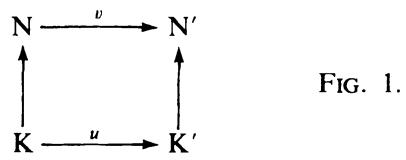
\includegraphics[keepaspectratio]{images/part002_8bfcf433.jpg}}

The mapping \(v^*\) is a homomorphism of \(\operatorname{Gal}(\mathbf{N}' / \mathbf{K}')\) into \(\operatorname{Gal}(\mathbf{N} / \mathbf{K})\) . For every \(x \in \mathbf{N}\) , the mapping \(\sigma \mapsto v^*(\sigma)(x) = v^{-1}(\sigma(v(x)))\) of \(\Gamma'\) into the discrete space \(\mathbf{N}\) is continuous, so \(v^*\) is continuous.

Three particular cases are of importance :

\begin{enumerate}
\def\labelenumi{\alph{enumi})}
\tightlist
\item
  If F is a Galois extension of K and E a subextension of F, we know (V, p.~67, Lemma 1) that F is a Galois extension of E. Let us apply what has been said to the case where N = F, \(K' = E\) , \(N' = F\) and \(v = Id_{F}\) . Then \(v^{*}\) is merely the canonical injection
\end{enumerate}

\[
j: \operatorname{Gal} (\mathrm{F} / \mathrm{E}) \rightarrow \operatorname{Gal} (\mathrm{F} / \mathrm{K}).
\]

This is sometimes called the inflation homomorphism.

\begin{enumerate}
\def\labelenumi{\alph{enumi})}
\setcounter{enumi}{1}
\tightlist
\item
  Suppose that in addition E is Galois over K. Let us apply what has been said to the case where N = E, \(K' = K\) , \(N' = F\) and v is the canonical injection of E into F. Then \(v^{*}\) is just the restriction homomorphism
\end{enumerate}

\[
\pi : \operatorname{Gal} (\mathrm{F} / \mathrm{K}) \rightarrow \operatorname{Gal} (\mathrm{E} / \mathrm{K}).
\]

We know (V, p.~60, Prop. 3) that \(\pi\) is surjective, with kernel \(\operatorname{Gal}(\mathrm{F} / \mathrm{E})\) and that by taking quotients it defines a topological group isomorphism of \(\operatorname{Gal}(\mathrm{F} / \mathrm{K}) / \operatorname{Gal}(\mathrm{F} / \mathrm{E})\) onto \(\operatorname{Gal}(\mathrm{E} / \mathrm{K})\) (V, p.~68, Cor. 4).

\begin{enumerate}
\def\labelenumi{\alph{enumi})}
\setcounter{enumi}{2}
\tightlist
\item
  Suppose that \(v^{-1}(\mathbf{K}') = \mathbf{K}\) and \(\mathbf{N}' = \mathbf{K}'(v(\mathbf{N}))\) ; let us show that the homomorphism
\end{enumerate}

\[
v ^ {*}: \operatorname{Gal} \left(\mathrm{N} ^ {\prime} / \mathrm{K} ^ {\prime}\right)\rightarrow \operatorname{Gal} (\mathrm{N} / \mathrm{K}),
\]

is a topological group isomorphism, sometimes called translation. For the group \(\operatorname{Gal}(N'/K')\) is compact, the group \(\operatorname{Gal}(N/K)\) is separated and \(v^{*}\) is continuous; so it is enough (Gen.~Top., I, p.~87, Cor. 2) to prove that \(v^{*}\) is bijective. Now every element \(\sigma\) of the kernel of \(v^{*}\) is an automorphism of \(N'\) which induces the identity on \(K'\) and on \(v(N)\) , hence \(\sigma = \varepsilon\) because \(\mathrm{N}' = \mathrm{K}'(v(N))\) ; it follows that \(v^{*}\) is injective. Further, the image of \(v^{*}\) is a closed subgroup \(\Delta\) of \(\operatorname{Gal}(N/K)\) .

(Gen.~Top., I, p.~81, ibid.) and the field of invariants of \(\Delta\) is equal to \(v^{-1}(\mathbf{K}') = \mathbf{K}\) ; therefore we have \(\Delta = \operatorname{Gal}(\mathbf{N}/\mathbf{K})\) (V, p.~67, Th. 4) and so \(v^{*}\) is surjective.

The general case may be reduced to the preceding ones by composition. To begin with we note that \(\mathrm{K}^{\prime}(v(\mathrm{N}))\) is the field of invariants in \(N^{\prime}\) of the kernel \(\Delta\) of \(v^{*}\) ; since \(\Delta\) is a normal subgroup of \(\operatorname{Gal}(\mathrm{N}^{\prime}/\mathrm{K}^{\prime})\) , the extension \(\mathrm{K}^{\prime}(v(\mathrm{N}))\) of \(K^{\prime}\) is Galois (V, p.~68, Cor. 4). Thus \(v^{*}\) is composed of the homomorphisms

\[
\operatorname{Gal} \left(\mathrm{N} ^ {\prime} / \mathrm{K} ^ {\prime}\right)\rightarrow \operatorname{Gal} \left(\mathrm{K} ^ {\prime} (v (\mathrm{N})) / \mathrm{K} ^ {\prime}\right) \stackrel {{\psi}} {{\rightarrow}} \operatorname{Gal} \left(\mathrm{N} / v ^ {- 1} \left(\mathrm{K} ^ {\prime}\right)\right) \stackrel {{j}} {{\rightarrow}} \operatorname{Gal} (\mathrm{N} / \mathrm{K});
\]

in this sequence \(\pi\) is the restriction homomorphism associated with the triple \(\mathbf{K}' \subset \mathbf{K}'(v(\mathbf{N})) \subset \mathbf{N}'\) , \(\psi\) is the translation isomorphism associated with the central square of the diagram (Fig. 2) and \(j\) is the inflation homomorphism associated with the triple \(\mathbf{K} \subset v^{-1}(\mathbf{K}') \subset \mathbf{N}\) .

The next theorem gives more detailed information about the structure of translation isomorphisms.

\[
\begin{array}{c}\mathbf {N} \rightarrow \mathbf {K} ^ {\prime} (v (\mathbf {N})) \rightarrow \mathbf {N} ^ {\prime}\\\uparrow \quad \uparrow\\\mathbf {K} \rightarrow v ^ {- 1} (\mathbf {K} ^ {\prime}) \rightarrow \mathbf {K} ^ {\prime}\end{array}\tag {FIG.2.}
\]

THEOREM 5. --- Let N' be an extension of K generated by two subextensions K' and N. Suppose that N is Galois over K, with Galois group Γ and that K' ∩ N = K. Then the extension N' of K' is Galois and the canonical homomorphism φ of K' ⊗K N into N' is an isomorphism. Let σ ∈ Gal(N/K) and let σ' be the element of Gal(N'/K') which corresponds to it under the translation isomorphism; then we have σ'∘φ = φ∘(Id\_\{K'\} ⊗σ).

We have \(N' = K'(N)\) and N is algebraic and separable over K; hence (V, p.~42, Prop. 10), the extension \(N'\) of \(K'\) is algebraic and separable. By Cor. 4 of V, p.~54 the extension \(N'\) of \(K'\) is quasi-Galois. Therefore the extension \(N'\) of \(K'\) is Galois. By c) above the mapping \(\sigma \mapsto \sigma | N\) is an homomorphism \(\lambda\) of \(\operatorname{Gal}(N'/K')\) onto \(\operatorname{Gal}(N/K)\) .

We have \(N = K'\) {[}N{]} because N is algebraic over K (V, p.~18, Cor. 1), hence \(\varphi\) is surjective. If \(\sigma\) belongs to \(\operatorname{Gal}(N/K)\) , we have

\[
\lambda^ {- 1} (\sigma) \circ \varphi = \varphi \circ \left(\operatorname{Id} _ {\mathrm{K} ^ {\prime}} \otimes \sigma\right).\tag{9}
\]

Therefore the kernel of \(\varphi\) is stable under the mappings \(\mathrm{Id}_{\mathbf{K}'} \otimes \sigma\) , hence of the form \(\mathbf{K}' \otimes_{\mathbf{K}} \mathbf{N}_0\) with \(\mathbf{N}_0 \subset \mathbf{N}\) (V, p.~63, Cor.). For \(x\) in \(\mathbf{N}_0\) we have \(x = \varphi(1 \otimes x) = 0\) , hence \(\mathbf{N}_0 = 0\) and so \(\varphi\) is injective.

COROLLARY 1. --- Let E' be a subfield of N' containing K'. There exists a unique subfield E of N containing K and such that E' = K'(E). We have E = E' ∩ N.

Put \(E = E' \cap N\) , then \(E' \supset K'(E)\) . Now put \(\Gamma = \text{Gal}(N/K)\) and \(\Delta = \text{Gal}(N/E)\) , and define \(\Gamma'\) and \(\Delta'\) similarly. The mapping \(\lambda : \sigma \mapsto \sigma | N\) is an isomorphism of \(\Gamma'\) onto \(\Gamma\) and also of \(\Delta'\) onto \(\Delta\) ; in other words, \(\Delta'\) consists of those \(\sigma \in \Gamma'\) for which \(\lambda(\sigma)\) belongs to \(\Delta\) . If \(\sigma \in \Gamma'\) leaves the elements of \(K'(E)\) fixed, we have \(\lambda(\sigma) \in \Delta\) , whence \(\sigma \in \Delta'\) and \(\sigma\) leaves the elements of \(E'\) fixed; by Cor. 1 of V, p.~68 we thus have \(K'(E) \supset E'\) .

We have proved the equality \(E' = K'(E)\) , whence \(\varphi^{-1}(E') = K' \otimes_{K} E\) . If F is a subfield of N containing K and such that \(E' = K'(F)\) , we have likewise \(\varphi^{-1}(E') = K' \otimes_{K} F\) , whence F = E.

COROLLARY 2. --- Let N be a Galois extension of K. Suppose that the Galois group \(\Gamma\) of N over K is the direct product of two closed subgroups \(\Gamma_1\) and \(\Gamma_2\) and denote by \(E_i\) the field of invariants of \(\Gamma_i\) for \(i = 1, 2\) . Then the canonical homomorphism of \(E_1 \otimes_K E_2\) into N is an isomorphism.

We have \(E_{1} \cap E_{2} = K\) and \(N = K(E_{1} \cup E_{2})\) by Cor. 6 (V, p.~69), and so it is enough to apply Theorem 5.

Remark. --- Let K and \(K'\) be two fields and u a homomorphism of K into \(K'\) . Let \(K_s\) (resp. \(K_s'\) ) be a separable closure (V, p.~45, Prop. 14) of K (resp. \(K'\) ) and \(\Pi\) (resp. \(\Pi'\) ) the Galois group of \(K_s\) over K (resp. \(K_s'\) over \(K'\) ). Since \(K_s\) is a separable algebraic extension of K and the extension ( \(K_s'\) , u) of K is separably closed, there exists (V, p.~45, Cor.) a homomorphism v of \(K_s\) into \(K_s'\) extending u. From v we obtain a continuous homomorphism \(v^*\) of \(\Pi'\) into \(\Pi\) . Let \(v_1\) be another extension of u; since \(K_s\) is a quasi-Galois extension of K, there exists an element \(\sigma_0\) of \(\Pi\) such that \(v_1 = v \circ \sigma_0\) . We conclude that \(v_1^*(\tau) = \sigma_0^{-1} v^*(\tau) \sigma_0\) for all \(\tau \in \Pi\) .

\subsection{The normal basis theorem}

Let N be a Galois extension of K, with Galois group \(\Gamma\) . We identify \(\Gamma\) with the canonical basis of the group algebra \(\mathbf{K}^{(\Gamma)}\) (III, p.~446); then N may be considered as a left \(\mathbf{K}^{(\Gamma)}\) -module (III, p.~447, Example), so that

\[
u. x = \sum_ {\sigma \in \Gamma} a _ {\sigma} \sigma (x) \quad \text { for } \quad x \in \mathbf {N} \quad \text { and } \quad u = \sum_ {\sigma \in \Gamma} a _ {\sigma} \sigma \quad \text { in } \quad \mathbf {K} ^ {(\Gamma)}.
\]

If \(\mathbf{N}\) is of finite degree over \(\mathbf{K}\) , the group \(\Gamma\) is finite by Dedekind's theorem (V, p.~27, Cor. 2) and we can define the element \(t = \sum_{\sigma \in \Gamma} \sigma\) in \(\mathbf{K}^{(\Gamma)}\) ; then we have

\[
\operatorname{Tr} _ {N / K} (x) = \sum_ {\sigma \in \Gamma} \sigma (x),
\]

that is, \(\operatorname{Tr}_{\mathbf{N} / \mathbf{K}}(x) = t.x\) for all \(x \in \mathbf{N}\) .

Let us define an action on the right by \(\Gamma\) on \(\mathbf{N}\) by \(x^{\sigma} = \sigma^{-1}(x)\) . In a similar way we can consider the multiplicative group \(\mathbf{N}^{*}\) as a right \(\mathbf{Z}^{(\Gamma)}\) -module, the external law being written \((x, u) \mapsto x^u\) . For example, the notation \(x^{2\sigma + 3\tau + \pi}\) , where \(\sigma, \tau, \pi\) are elements of \(\Gamma\) , indicates the product \((x^\sigma)^2 \cdot (x^\tau)^3 \cdot x^\pi\) . If \(\mathbf{N}\) is of finite degree over \(\mathbf{K}\) and \(t = \sum_{\sigma \in \Gamma} \sigma\) as above, then we have \(\mathrm{N}_{\mathrm{N/K}}(x) = \prod_{\sigma \in \Gamma} x^\sigma\) , that is, \(\mathrm{N}_{\mathrm{N/K}}(x) = x^t\) for all \(x \in \mathbf{N}^*\) .

Suppose henceforth that N is of finite degree over K. Given \(x \in N\) , for \(\{x\}\) to be a basis of the \(\mathbf{K}^{(\Gamma)}\) -module N it is necessary and sufficient that the family \((\sigma(x))_{\sigma \in \Gamma}\) should be a basis of N over K. Such a basis is called a normal basis of N over K.

THEOREM 6. --- Let N be a Galois extension of finite degree over K and let \(\Gamma\) be the Galois group of N over K. Then there exists a normal basis of N over K; in other words, the \(\mathbf{K}^{(\Gamma)}\) -module N is free of rank 1.

We shall give two proofs of this statement. The first uses the following lemma which will be proved in Chapter VIII (§ 2, No.~5).

* Lemma 3. --- Let A be a K-algebra, \(\mathbf{M}_1\) and \(\mathbf{M}_2\) two A-modules of finite rank over K and suppose that there exists an extension L of K such that the modules \(\mathrm{L} \otimes_{\mathrm{K}} \mathrm{M}_1\) and \(\mathrm{L} \otimes_{\mathrm{K}} \mathrm{M}_2\) over the ring \(\mathrm{L} \otimes_{\mathrm{K}} \mathrm{A}\) are isomorphic. Then the A-modules \(\mathbf{M}_1\) and \(\mathbf{M}_2\) are isomorphic.

We shall apply Lemma 3 in the case where \(\mathbf{A} = \mathbf{K}^{(\Gamma)}\) , \(\mathbf{M}_1 = \mathbf{N}\) , \(\mathbf{M}_2 = \mathbf{A}_s\) and \(\mathbf{L} = \mathbf{N}\) . By the Cor. of V, p.~64 there exists a K-isomorphism \(\varphi\) of \(\mathbf{N} \otimes_{\mathbf{K}} \mathbf{N}\) onto \(\mathbf{N} \otimes_{\mathbf{K}} \mathbf{K}^{(\Gamma)}\) which maps \(x \otimes y\) to \(\sum x \sigma^{-1}(y) \otimes \sigma\) . It is clear that \(\varphi\) is an isomorphism of \(\mathbf{N} \otimes_{\mathbf{K}} \mathbf{K}^{(\Gamma)}\) -modules and so the theorem follows from Lemma 3. *

For the second proof we shall use the following proposition :

PROPOSITION 10. --- Let \(x \in \mathbb{N}\) , then for \(\{x\}\) to form a basis of the \(K^{(\Gamma)}\) -module \(\mathbb{N}\) it is necessary and sufficient that \(\det(\sigma\tau(x))_{\sigma,\tau \in \Gamma} \neq 0\) .

Since \(\mathbf{K}^{(\Gamma)}\) and \(\mathbf{N}\) have the same dimension over \(\mathbf{K}\) , to say that \(\{x\}\) is a basis of \(\mathbf{N}\) over \(\mathbf{K}^{(\Gamma)}\) means that the mapping \(a \mapsto ax\) of \(\mathbf{K}^{(\Gamma)}\) into \(\mathbf{N}\) is injective. This in turn means that the mapping \(b \mapsto b(1 \otimes x)\) of \(\mathbf{N} \otimes_{\mathbf{K}} \mathbf{K}^{(\Gamma)}\) into \(\mathbf{N} \otimes_{\mathbf{K}} \mathbf{N}\) is injective (II, p.~306, Prop. 14). Now there is an \(\mathbf{N} \otimes_{\mathbf{K}} \mathbf{K}^{(\Gamma)}\) -module isomorphism of \(\mathbf{N} \otimes_{\mathbf{K}} \mathbf{N}\) onto \(\mathbf{N} \otimes_{\mathbf{K}} \mathbf{K}^{(\Gamma)}\) which maps \(1 \otimes x\) to \(\sum_{\sigma} \sigma^{-1}(x) \otimes \sigma\) . It follows that \(\{x\}\) is a basis

of N over \(\mathbf{K}^{(\Gamma)}\) if and only if, for every non-zero family of elements \((n_{\tau})_{\tau\in\mathrm{T}}\) of N we have \(\left(\sum n_{\tau}\otimes\tau\right)\left(\sum\sigma^{-1}(x)\otimes\sigma\right)\neq0\) . But this last relation means that there exists \(\sigma\in\Gamma\) such that \(\sum_{\tau}n_{\tau}\sigma^{-1}\tau(x)\neq0\) , whence the proposition.

\begin{enumerate}
\def\labelenumi{\Alph{enumi})}
\tightlist
\item
  Suppose that K is infinite; the mapping \(x \mapsto \det(\sigma\tau(x))\) of N into N is a polynomial mapping over K (IV, p.~54). By extension of scalars from K to N we get a corresponding mapping for the vector N-space \(\mathbf{N} \otimes_{\mathbf{K}} \mathbf{N}\) and we have just seen that the latter is not identically zero (because \(\mathbf{N} \otimes_{\mathbf{K}} \mathbf{N}\) is free of rank 1 over \(\mathbf{N} \otimes_{\mathbf{K}} \mathbf{K}^{(\Gamma)}\) ). So there exists \(x \in \mathbf{N}\) such that \(\det(\sigma\tau(x)) \neq 0\) (IV, p.~18, Th. 2); more generally, from the same reference we have:
\end{enumerate}

PROPOSITION 11. --- Suppose that K is infinite and let P:N→K be a polynomial mapping which is non-zero on K. There exists x∈N such that P(x)≠0 and \{x\} is a basis of N over K \(^{(\Gamma)}\) .

\begin{enumerate}
\def\labelenumi{\Alph{enumi})}
\setcounter{enumi}{1}
\tightlist
\item
  Suppose that K is finite. By Prop. 4 (V, p.~95) \(^{1}\) every extension of finite degree over K has a cyclic Galois group. We shall therefore more generally consider the case where the group \(\Gamma\) is cyclic of order n; we denote by \(\gamma\) a generator of \(\Gamma\) .
\end{enumerate}

The following lemma is a particular case of more general results proved in Chapter VII. The ring A is either the ring Z of rational integers or the ring K{[}X{]} of polynomials over the field K.

Lemma 4. --- Let M be a torsion A-module generated by a finite number \(x_{1}, \ldots, x_{h}\) of elements; then there exists an element x of M whose annihilator (II, p.~219) is equal to the annihilator of M.

In both cases A is an integral domain and every ideal of A is principal. When A = Z (resp. A = K{[}X{]}), we denote by P the set of prime numbers (resp. the set of irreducible monic polynomials in K{[}X{]}). For every element \(a \neq 0\) of A there exists then an invertible element u of A and a family \((v_{p}(a))_{p \in \mathcal{P}}\) , with finite support, of positive integers such that \(a = u \prod_{p \in \mathcal{P}} p^{v_{p}(a)}\) and u and the integers

\(v_{p}(a)\) are uniquely determined (I, p.~51 and IV, p.~13, Prop. 13).

Let \(\mathfrak{a}_i\) be the annihilator of \(x_i\) (for \(1 \leqslant i \leqslant h\) ) and \(\mathfrak{a}\) the annihilator of \(\mathbf{M}\) ; let \(a_1, \ldots, a_h\) , \(a\) be non-zero elements of \(\mathbf{A}\) such that \(\mathfrak{a}_i = \mathbf{A}a_i\) and \(\mathfrak{a} = \mathbf{A}a\) ; since \(\mathfrak{a} = \mathfrak{a}_1 \cap \ldots \cap \mathfrak{a}_h\) , it follows from what has been said that

\[
v _ {p} (a) = \sup _ {1 \leqslant i \leqslant h} v _ {p} (a _ {i}) \quad \text { for   all } p \in \mathscr {P}.\tag{10}
\]

Let us write \(a\) in the form \(up_1^{n(1)} \ldots p_r^{n(r)}\) , with \(p_1, \ldots, p_r\) distinct in \(\mathcal{P}\) , \(n(1) > 0, \ldots, n(r) > 0\) and \(u\) an invertible element of \(A\) . Let \(j = 1, \ldots, r\) ; by (10) there exists an integer \(c(j)\) such that \(1 \leqslant c(j) \leqslant h\) and \(v_{p_j}(a_{c(j)}) = n(j)\) ; there exists \(b_j\) in \(A\) with \(a_{c(j)} = p_j^{n(j)}b_j\) and the element \(y_j = b_jx_{c(j)}\) has as annihilator the ideal \(Ap_j^{n(j)}\) .

Let us show that the annihilator b of \(y = y_{1} + \cdots + y_{r}\) is equal to the annihilator a of M. In any case we have \(a \subset b\) , so b is of the form \(Ap_{1}^{m(1)} \ldots p_{r}^{m(r)}\) with \(0 \leqslant m(j) \leqslant n(j)\) for \(1 \leqslant j \leqslant r\) . If we had \(a \neq b\) , there would exist an integer j such that \(1 \leqslant j \leqslant r\) and \(m(j) < n(j)\) , and hence \(d_{j} = a/p_{j}\) would annihilate y. Now we have \(d_{j}y_{k} = 0\) for \(k \neq j\) , whence we obtain \(d_{j}y_{j} = 0\) ; but the annihilator of \(y_{j}\) is \(Ap_{j}^{m(j)}\) and \(d_{j}\) is not a multiple of \(p_{j}^{m(j)}\) . So the hypothesis \(a \neq b\) is absurd.

We shall apply Lemma 4 to the case where \(\mathbf{A}\) is the polynomial ring \(\mathbf{K}[\mathbf{X}]\) and \(\mathbf{M}\) the abelian group \(\mathbf{N}\) with the external law defined by \(a \cdot x = \sum_{k=0}^{\infty} c_k \gamma^k(x)\) for \(a = \sum_{k=0}^{\infty} c_k \mathbf{X}^k\) in \(\mathbf{K}[\mathbf{X}]\) and \(x \in \mathbb{N}\) . Let \(\mathfrak{a}\) be the annihilator of \(\mathbf{M}\) , then \(\gamma^n = 1\) , hence the polynomial \(\mathbf{X}^n - 1\) lies in \(\mathfrak{a}\) . Let \(\mathbf{F} \in \mathfrak{a}\) ; by IV, p.~11, Cor. there exist elements \(c_0, c_1, \ldots, c_{n-1}\) of \(\mathbf{K}\) and \(\mathbf{G} \in \mathbf{K}[\mathbf{X}]\) such that

\[
\mathrm{F} (\mathbf {X}) = c _ {0} + c _ {1} \mathbf {X} + \dots + c _ {n - 1} \mathbf {X} ^ {n - 1} + (\mathbf {X} ^ {n} - 1) \mathrm{G} (\mathbf {X}).\tag{11}
\]

Thus we have \(c_{0} + c_{1}\gamma + \cdots + c_{n-1}\gamma^{n-1} = 0\) in \(\operatorname{Hom}_{\mathbf{K}}(\mathbf{N}, \mathbf{N})\) and since the automorphisms 1, \(\gamma\) , \(\gamma^{2}\) , \ldots, \(\gamma^{n-1}\) of N are distinct, Dedekind's theorem (V, p.~27, Cor. 2) implies that \(c_{0} = c_{1} = \cdots = c_{n-1} = 0\) . Finally, we have

\[
\mathrm{F} (\mathbf {X}) = \left(\mathbf {X} ^ {n} - 1\right) \mathrm{G} (\mathbf {X}), \quad \text { that   is }, \quad \mathfrak {a} = \left(\mathbf {X} ^ {n} - 1\right) \mathrm{K} [ \mathbf {X} ].
\]

By Lemma 4 there exists an element \(x\) of \(\mathbf{N}\) whose annihilator in \(\mathbf{K}[\mathbf{X}]\) is equal to \((\mathbf{X}^n - 1)\mathbf{K}[\mathbf{X}]\) . Since the monomials 1, \(\mathbf{X}, \ldots, \mathbf{X}^{n-1}\) form a basis of a vector subspace of \(\mathbf{K}[\mathbf{X}]\) supplementary to \((\mathbf{X}^n - 1)\mathbf{K}[\mathbf{X}]\) (IV, p.~11, Cor.), the elements \(x, \gamma(x), \ldots, \gamma^{n-1}(x)\) of \(\mathbf{N}\) are linearly independent over \(\mathbf{K}\) . Since \([\mathbf{N}:\mathbf{K}] = n(\mathbf{V},\mathbf{p}.66,\mathbf{Th}.3)\) , the sequence \((x,\gamma(x),\ldots,\gamma^{n-1}(x))\) is therefore a (normal) basis of \(\mathbf{N}\) over \(\mathbf{K}\) .

\subsection{\texorpdfstring{Finite \(\Gamma\)-sets and etale algebras}{Finite Gamma-sets and etale algebras}}

Let \(K_s\) be a separable closure of \(K\) (V, p.~45, Prop. 14) and \(\Gamma\) the Galois group of \(K_s\) over \(K\) . By a \(\Gamma\) -set we understand a set \(X\) with an action \((\sigma, x) \mapsto \sigma x\) of the group \(\Gamma\) such that the stabilizer of each point of \(X\) is an open subgroup of \(\Gamma\) . It comes to the same to say that the mapping \((\sigma, x) \mapsto \sigma x\) of \(\Gamma \times X\) into \(X\) is continuous when \(X\) is equipped with the discrete topology.

Let \(\mathbf{X}\) be a finite \(\Gamma\) -set. We define an action of \(\Gamma\) on the K-algebra \(\mathbf{K}_s^{\mathbf{X}}\) of mappings of \(\mathbf{X}\) into \(\mathbf{K}_s\) by the formula

\[
u _ {\sigma} f (x) = \sigma \left(f \left(\sigma^ {- 1} x\right)\right)\tag{12}
\]

for \(\sigma \in \Gamma\) , \(f \in \mathbf{K}_s^X\) and \(x \in \mathbf{X}\) . Let \(\Theta(\mathbf{X})\) be the set of invariants of \(\Gamma\) in \(\mathbf{K}_s^X\) ; this is the sub-K-algebra of \(\mathbf{K}_s^X\) consisting of mappings \(f: \mathbf{X} \to \mathbf{K}_s\) such that \(f(\sigma x) = \sigma(f(x))\) for \(\sigma \in \Gamma\) and \(x \in \mathbf{X}\) .

Lemma 5. --- Let X be a finite \(\Gamma\) -set and let \(x_1, \ldots, x_n\) be points of X such that the orbits \(\Gamma x_1, \ldots, \Gamma x_n\) form a partition of X. For \(1 \leqslant i \leqslant n\) let \(\Delta_i\) be the stabilizer of \(x_i\) in \(\Gamma\) and let \(L_i\) be the field of invariants of \(\Delta_i\) . Then \(L_1, \ldots, L_n\) are separable extensions of finite degree of K, and the mapping \(f \mapsto (f(x_1), \ldots, f(x_n))\) is a K-algebra isomorphism of \(\Theta(X)\) onto \(L_1 \times \cdots \times L_n\) .

By hypothesis the subgroups \(\Delta_{1},\ldots,\Delta_{n}\) of \(\Gamma\) are open and Cor. 5 of V, p.~68, shows that the subextensions \(L_{1},\ldots,L_{n}\) of \(K_{s}\) are of finite degree over K. Clearly they are separable; now the last assertion of Lemma 5 is immediate.

From Lemma 5 and Th. 4 (V, p.~34f.) we obtain immediately the following result.

PROPOSITION 12. --- For every finite \(\Gamma\) -set X the algebra \(\Theta(X)\) is etale over K, of degree equal to the cardinal of X. Moreover, every etale algebra over K is isomorphic to an algebra of the form \(\Theta(X)\) .

Remarks. --- a) It is easy to show that for every K-algebra homomorphism \(\varphi\) of \(\Theta(\mathbf{X})\) into \(\mathbf{K}_s\) there exists a unique element \(x\) of \(\mathbf{X}\) such that \(\varphi(f) = f(x)\) for all \(f \in \Theta(\mathbf{X})\) .

\begin{enumerate}
\def\labelenumi{\arabic{enumi})}
\setcounter{enumi}{1}
\tightlist
\item
  Let X and Y be two finite \(\Gamma\) -sets. Let \(\mathfrak{F}_{\Gamma}(X, Y)\) be the set of mappings \(u\) of X into Y such that \(u(\sigma x) = \sigma u(x)\) for all \(\sigma \in \Gamma\) and all \(x \in X\) . For \(u \in \mathfrak{F}_{\Gamma}(X, Y)\) we define a K-algebra homomorphism \(u^{*}: \Theta(Y) \to \Theta(X)\) by \(u^{*}(f) = f \circ u\) . For every homomorphism \(\Psi\) of \(\Theta(Y)\) into \(\Theta(X)\) there exists a unique element \(u\) of \(\mathfrak{F}_{\Gamma}(X, Y)\) such that \(\Psi = u^{*}\) .
\end{enumerate}

\subsection{The structure of quasi-Galois extensions}

PROPOSITION 13. --- Let N be a quasi-Galois extension of K. We denote by \(N_{r}\) the field of invariants of the group of all K-automorphisms of N and by \(N_{s}\) the relative separable algebraic closure of K in N (V, p.~44). Then :

\begin{enumerate}
\def\labelenumi{\alph{enumi})}
\item
  \(\mathbf{N}_r\) is the relative \(p\) -radical closure of \(\mathbf{K}\) in \(\mathbf{N}\) (V, p.~25).
\item
  \(N_{s}\) is a Galois extension of K and every K-automorphism of \(N_{s}\) extends in a unique fashion to an \(N_{r}\) -automorphism of N.
\item
  The fields \(\mathbf{N}_r\) and \(\mathbf{N}_s\) are linearly disjoint over \(\mathbf{K}\) and we have \(\mathbf{N} = \mathbf{K}[\mathbf{N}_r \cup \mathbf{N}_s]\) ; in other words, the canonical homomorphism of \(\mathbf{N}_r \otimes_{\mathbf{K}} \mathbf{N}_s\) into \(\mathbf{N}\) is an isomorphism.
\end{enumerate}

Let \(\Omega\) be an algebraic closure of K containing N as subextension (V, p.~23, Th. 2). Every K-automorphism of \(\Omega\) induces an automorphism of N because N is quasi-Galois. Therefore every element of \(N_r\) is invariant under the group of K-automorphisms of \(\Omega\) , hence \(p\) -radical over K (V, p.~53, Cor. 3). Conversely every element of N which is \(p\) -radical over K is clearly invariant under every K-automorphism of N and hence belongs to \(N_r\) . This proves \(a\) ).

Every K-automorphism of \(\Omega\) maps N into N, hence \(N_s\) into \(N_s\) , so \(N_s\) is a quasi-Galois extension of K (V, p.~54, Prop. 3). It follows that \(N_s\) is a Galois extension of K. Every element of \(N_r \cap N_s\) is separable algebraic and \(p\) -radical over K, hence belongs to K (V, p.~Cor. 3); we thus have \(K_r \cap K_s = K\) . Now N is \(p\) -radical over \(N_s\) (V, p.~44, Prop. 13) and separable algebraic over \(N_r\) (V, p.~56, Th. 1) hence both \(p\) -radical and separable over \(K(N_r \cup N_s)\) . Hence we have \(N = K(N_r \cup N_s)\) (V, p.~39, Cor. 3) and the assertions \(b\) , \(c\) ) follow from Th. 5 (V, p.~71).

COROLLARY. --- Let p the characteristic exponent of K, \(\bar{K}\) an algebraic closure of K, \(K_{s}\) the relative separable closure of K in \(\bar{K}\) and \(K^{p^{-\infty}}\) the perfect closure of K. Then the canonical homomorphism of \(K^{p^{-\infty}} \otimes K_{s}\) into \(\bar{K}\) is an isomorphism.

Remark. --- Let R (resp. S) be a p-radical (resp. separable algebraic) extension of K. Then the algebra \(R \otimes_{K} S\) is a field : for R (resp. S) is isomorphic to a subextension of \(K^{p^{-\infty}}\) (resp. \(K_{s}\) ) and it suffices to apply the above Cor. and Prop. 1 of V, p.~17.

\section{ABELIAN EXTENSIONS}

Throughout this paragraph K denotes a field.

\subsection{Abelian extensions and the abelian closure}

DEFINITION 1. --- An extension E of K is said to be abelian if it is Galois and its Galois group is commutative.

Since every subgroup of a commutative group is normal, Cor. 4 of V, p.~68 shows that every subextension of an abelian extension is abelian.

PROPOSITION 1. --- Let E be a Galois extension of K and Γ its Galois group. Let Δ be the derived group of Γ (I, p.~10, Def. 4) and F the field of invariants of Δ. For a subextension L to E to be abelian it is necessary and sufficient that it should be contained in F.

Firstly we note that F is also the field of invariants of the closure \(\bar{\Delta}\) of \(\Delta\) in \(\Gamma\) , and that \(\bar{\Delta}\) is a closed normal subgroup of \(\Gamma\) . By V, p.~68, Cor. 4, F is thus a Galois extension of K. Further, the Galois group of F over K is isomorphic to \(\Gamma/\bar{\Delta}\) and hence is commutative. Hence every subextension of F is abelian. Conversely let L be an abelian extension of K contained in E, and let \(\Pi\) be the Galois group of E over L. Since L is Galois, \(\Pi\) is a normal subgroup of \(\Gamma\) and the Galois group of L over K is isomorphic to \(\Gamma/\Pi\) (V, p.~68, Cor. 4). Therefore \(\Gamma/\Pi\) is commutative and \(\Pi\) contains \(\Delta\) , whence \(L \subset F\) .

COROLLARY. --- Let E be an extension of K and let \((\mathrm{E}_{i})_{i\in I}\) be a family of subextensions of E such that \(\mathrm{E}=\mathrm{K}\left(\bigcup_{i\in I}\mathrm{E}_{i}\right)\) . Suppose that each extension

\(E_{i}\) is abelian, then the same is true of E.

In the first place E is a Galois extension of K (V, p.~57, Prop. 1). If the field F is defined as in Prop. 1, then we have \(E_{i} \subset F\) for all \(i \in I\) , whence E = F.

An extension E of K is said to be an abelian closure of K if it is an abelian extension of K and every abelian extension of K is isomorphic to a subextension of E. Prop. 1 implies the existence of an abelian closure of K: for let \(K_{s}\) be a separable closure of K, with Galois group \(\Gamma\) and let \((\overline{\Gamma},\overline{\Gamma})\) be the closure of the derived group of \(\Gamma\) ; denote by \(K_{ab}\) the field of invariants of \((\overline{\Gamma},\overline{\Gamma})\) ; since every separable algebraic extension of K is isomorphic to a subextension of \(K_{s}\) (V, p.~45, Cor.). Prop. 1 shows that \(K_{ab}\) is an abelian closure of K. The Galois group of \(K_{ab}\) over K is canonically isomorphic to \(\Gamma/(\overline{\Gamma},\overline{\Gamma})\) . Let us now show the uniqueness of abelian closures: let E, \(E'\) be two abelian closures of K; by definition there exist K-homomorphisms \(u:E\to E'\) and \(v:E'\to E\) and Prop. 1 (V, p.~52) implies that \(v(u(E)) = E\) and \(u(v(E')) = E'\) , hence \(u\) is a K-isomorphism of \(E\) onto \(E'\) . Any other K-isomorphism of \(E\) onto \(E'\) is of the form \(u_1 = \sigma_0 \circ u\) with \(\sigma_0 \in \operatorname{Gal}(E'/K)\) ; since \(\operatorname{Gal}(E'/K)\) is commutative, the isomorphism \(\sigma \mapsto u \circ \sigma \circ u^{-1}\) of \(\operatorname{Gal}(E/K)\) onto \(\operatorname{Gal}(E'/K)\) is independent of \(u\) ; it is called the canonical isomorphism of \(\operatorname{Gal}(E/K)\) onto \(\operatorname{Gal}(E'/K)\) .

\subsection{Roots of unity}

DEFINITION 2. --- An element \(\zeta\) of \(\mathbf{K}\) is said to be a root of unity if there exists an integer \(n > 0\) such that \(\zeta^n = 1\) ; for every integer \(n > 0\) such that \(\zeta^n = 1\) , \(\zeta\) is called an \(n\) -th root of unity.

It amounts to the same to say that the roots of unity are the elements of finite order of the multiplicative group \(K^{*}\) of non-zero elements of K (I, p.~51). The roots of unity form a subgroup \(\mu_{\infty}(\mathbf{K})\) of \(K^{*}\) , the n-th roots form a subgroup \(\mu_{n}(\mathbf{K})\) of \(\mu_{\infty}(\mathbf{K})\) . We have \(\mu_{\infty}(\mathbf{K}) = \bigcup_{n \geqslant 1} \mu_{n}(\mathbf{K})\) and \(\mu_{n}(\mathbf{K}) \subset \mu_{m}(\mathbf{K})\) if n divides

\begin{enumerate}
\def\labelenumi{\alph{enumi}.}
\setcounter{enumi}{12}
\tightlist
\item
  For every root of unity \(\zeta\) there exists a least integer \(n \geqslant 1\) such that \(\zeta\) belongs to \(\mu_{n}(\mathbf{K})\) , namely the order of \(\zeta\) in the group \(K^{*}\) .
\end{enumerate}

The group \(\mu_n(\mathbf{K})\) , being the set of roots of the polynomial \(\mathbf{X}^n - 1\) , is of finite order \(\leqslant n\) . Let \(p\) be the characteristic of \(\mathbf{K}\) . When \(p = 0\) , or when \(p \neq 0\) and \(n\) is not divisible by \(p\) , the derivative \(n\mathbf{X}^{n-1}\) of \(\mathbf{X}^n - 1\) is relatively prime to \(\mathbf{X}^n - 1\) and so the polynomial \(\mathbf{X}^n - 1\) is then separable; if moreover \(\mathbf{K}\) is algebraically closed, \(\mu_n(\mathbf{K})\) is thus a group of \(n\) elements.

Suppose that K is of non-zero characteristic p and let \(r \geqslant 0\) be an integer; since the mapping \(x \mapsto x^{p^{r}}\) of K into K is injective, we have \(\mu_{np^{r}}(\mathbf{K}) = \mu_n(\mathbf{K})\) for every integer \(n \geqslant 1\) .

We remark that a field may contain no \(n\) -th root of unity other than 1: this is the case for example with the prime fields \(\mathbf{Q}\) and \(\mathbf{F}_2\) for any odd integer \(n\) .

THEOREM 1. --- Let p be the characteristic exponent of K and let n \textgreater{} 0 be an integer. Then the group \(\mu_{n}(\mathbf{K})\) of n-th roots of unity in K is cyclic and its order divides n; when K is algebraically closed and n is prime to p, the group \(\mu_{n}(\mathbf{K})\) is cyclic of order n.

It is enough to prove the first assertion of the theorem which is a consequence of the following more precise lemma:

Lemma 1. --- Let G be a finite subgroup of \(\mathbf{K}^*\) of order \(m\) ; then G is cyclic and we have \(\mathrm{G} = \mu_m(\mathrm{K})\) .

Consider G as Z-module; we have mx = 0 for all \(x \in G\) , hence the annihilator of G is an ideal of the form rZ, where the integer \(r \geqslant 1\) divides m. We thus have \(G \subset \mu_{r}(K)\) . By Lemma 4 (V, p.~74) applied with A = Z and M = G there exists an element x of G of order r; let \(G'\) be the cyclic subgroup of G generated by x. We have \(G' \subset \mu_{r}(K)\) , Card \((G') = r\) and Card \(\mu_{r}(K) \leqslant r\) ; therefore we have

\(G' = \mu_r(K) \supset G\) and \(G\) is cyclic of order \(r\) , hence equal to \(\mu_r(K)\) . Since \(G\) has order \(m\) , we have \(m = r\) and the lemma follows.

PROPOSITION 2. --- Let K be algebraically closed and let p be its characteristic exponent. There exists an isomorphism of \(\mu_{\infty}(\mathbf{K})\) onto the group \(\mathbf{Q}/\mathbf{Z}[1/p]\) .

We have denoted by \(\mathbf{Z}[1/p]\) the subring of \(\mathbf{Q}\) generated by \(1/p\) , that is, the set of rational numbers of the form \(a/p^n\) with \(a \in \mathbf{Z}\) and \(n \geqslant 1\) ; thus we have \(\mathbf{Z}[1/p] = \mathbf{Z}\) if \(\mathbf{K}\) is of characteristic 0.

Let \((\nu_{n})_{n\geqslant 1}\) be the strictly increasing sequence consisting of all the integers which are not divisible by \(p\) , if \(p\neq 1\) ; put \(\lambda_{n} = \nu_{1}\nu_{2}\dots \nu_{n}\) and denote by \(\mathrm{H}_n\) the group of \(\lambda_{n}\) -th roots of unity; we have \(\mathrm{H}_{n + 1}\supset \mathrm{H}_n\) and \(\mu_{\infty}(\mathbf{K}) = \cup_{n}\mathrm{H}_{n}\) . Since \(\mathrm{H}_n\) is cyclic of order \(\lambda_{n}\) (Th. 1), there exists a sequence

\((\alpha_{n})_{n\geqslant 1}\) of roots of unity such that \(\alpha_{n}\) generates \(\mathrm{H}_n\) and \(\alpha_{n} = \alpha_{n + 1}^{\nu_{n + 1}}\)

Further let \(\beta_{n}\) be the residue class mod \(\mathbf{Z}[1/p]\) of \(1/\lambda_{n}\) and let \(\mathbf{H}_{n}^{\prime}\) be the cyclic subgroup of \(\mathbf{Q}/\mathbf{Z}[1/p]\) generated by \(\beta_{n}\) . It is clear that \(\beta_{n} = \nu_{n+1}\beta_{n+1}\) and \(\mathbf{H}_{n}^{\prime}\) is of order \(\lambda_{n}\) because \(\lambda_{n}\) is not divisible by \(p\) if \(p \neq 1\) . Thus there exists for all \(n \geqslant 1\) an isomorphism \(\varphi_{n}: \mathrm{H}_{n} \to \mathrm{H}_{n}^{\prime}\) such that \(\varphi_{n}(\alpha_{n}) = \beta_{n}\) and the relations \(\alpha_{n} = \alpha_{n+1}^{\nu_{n+1}}\) , \(\beta_{n} = \nu_{n+1}\beta_{n+1}\) show that \(\varphi_{n+1}\) extends \(\varphi_{n}\) . Finally there exists a unique isomorphism \(\varphi\) of \(\mu_{\infty}(\mathbf{K})\) onto \(\mathbf{Q}/\mathbf{Z}[1/p]\) extending the isomorphisms \(\varphi_{n}\) , that is, \(\varphi(\alpha_{n}) = \beta_{n}\) for all \(n \geqslant 1\) .

Remarks. --- 1) When K is an algebraically closed field of characteristic 0, the group \(\mu_{\infty}(\mathbf{K})\) is thus isomorphic (not canonically) to \(\mathbf{Q}/\mathbf{Z}\) . * When K is the field \(\mathbf{C}\) of complex numbers, we can write down an explicit such isomorphism; in effect the mapping \(x \mapsto e^{2\pi ix}\) is a homomorphism of \(\mathbf{Q}\) into \(\mathbf{C}^*\) with kernel \(\mathbf{Z}\) and image \(\mu_{\infty}(\mathbf{C})\) ; thus by passage to quotients it defines an isomorphism of \(\mathbf{Q}/\mathbf{Z}\) onto \(\mu_{\infty}(\mathbf{C})\) . *

\begin{enumerate}
\def\labelenumi{\arabic{enumi})}
\setcounter{enumi}{1}
\item
  The following result may be shown (cf.~V, p.~165, Ex. 21): let G and H be two commutative groups all of whose elements are of finite order. Suppose that for every integer \(n \geqslant 1\) , the equation \(nx = 0\) has the same number of solutions, assumed finite in G and in H. Then the groups G and H are isomorphic. This provides a new proof of Prop. 2.
\item
  For every prime number \(l\) put \(\mu_{l^{\infty}}(\mathbf{K}) = \bigcup_{n\geqslant 0}\mu_{l^{n}}(\mathbf{K})\) . When \(l\) is the characteristic
\end{enumerate}

\(p\) of \(\mathbf{K}\) , we have \(\mu_{p^{\infty}}(\mathbf{K}) = \{1\}\) . From I, p.~80, Th. 4, we deduce that \(\mu_{\infty}(\mathbf{K})\) is a direct sum of the subgroups \(\mu_{l^{\infty}}(\mathbf{K})\) , where \(l\) runs over the set of all prime numbers distinct from \(p\) . For a given prime number \(l\) only two cases are possible: either \(\mu_{l^{\infty}}(\mathbf{K})\) is finite and then \(\mu_{l^{\infty}}(\mathbf{K})\) is isomorphic to \(\mathbf{Z}/l^{n}\mathbf{Z}\) for a suitable \(n\) (Th. 1), or \(\mu_{l^{\infty}}(\mathbf{K})\) is infinite and then \(\mu_{l^{\infty}}(\mathbf{K})\) is isomorphic to \(\mathbf{Z}[l^{-1}]/\mathbf{Z}\) (cf.~Remark 2).

\subsection{Primitive roots of unity}

Let \(n \geqslant 1\) be an integer. By the Euler indicator of \(n\) , written \(\varphi(n)\) , we understand the number of invertible elements of the ring \(\mathbf{Z}/n\mathbf{Z}\) of integers modulo n.~By the next proposition \(\varphi(n)\) is also the number of integers k prime to n and such that \(0 \leqslant k < n\) .

PROPOSITION 3. --- Let k and \(n \geqslant 1\) be two integers. Then the following assertions are equivalent :

\begin{enumerate}
\def\labelenumi{\alph{enumi})}
\item
  the residue class of k mod n is invertible in the ring Z/nZ ;
\item
  the residue class of k mod n generates the cyclic group Z/nZ ;
\item
  the integers \(k\) and \(n\) are relatively prime (I, p.~112).
\end{enumerate}

Each of the conditions a) and b) means that there exists an integer x such that \(kx \equiv 1 \pmod{n}\) , that is, there exist two integers x and y such that \(kx + ny = 1\) . This latter condition just means that k and n are relatively prime.

COROLLARY 1. --- Let G be a cyclic group of order n and let d be a divisor of n.~Then the number of elements of order d in G is equal to \(\varphi(d)\) . In particular, \(\varphi(n)\) is the number of generators of G.

Since G is isomorphic to Z/nZ, the number of generators of G is equal to \(\varphi(n)\) by Prop. 3. Let g be a generator of G; then the elements h of G such that \(h^{d}=1\) constitute the subgroup H of G generated by \(g^{n/d}\) ; this group is cyclic of order d and the elements of order d of G are the generators of H, hence their number is \(\varphi(d)\) .

COROLLARY 2.--- For every integer \(n \geqslant 1\) , we have

\[
\sum_ {d \mid n} \varphi (d) = n,\tag{1}
\]

where the integer \(d\) runs over the set of divisors \(>0\) of \(n\) \(^{1}\) .

With the notation of Cor. 1, every element of G has a finite order which is a divisor d of n and for a fixed d there are \(\varphi(d)\) such elements.

The calculation of \(\varphi(n)\) is based on the two formulae:

\begin{enumerate}
\def\labelenumi{(\arabic{enumi})}
\setcounter{enumi}{1}
\item
  \(\varphi(mn) = \varphi(m)\varphi(n)\) if \(m\) and \(n\) are relatively prime,
\item
  \(\varphi(p^a) = p^{a-1}(p - 1)\) ( \(p\) prime, \(a \geqslant 1\) ).
\end{enumerate}

The first follows at once from the fact that the rings \(\mathbf{Z} / mn\mathbf{Z}\) and \((\mathbf{Z} / m\mathbf{Z}) \times (\mathbf{Z} / n\mathbf{Z})\) are isomorphic (I, p.~112), and that \((\mathbf{A} \times \mathbf{B})^{*} = \mathbf{A}^{*} \times \mathbf{B}^{*}\) for two rings A and B. To prove (3) we note that the positive divisors of \(p^{a}\) are 1, \(p\) , \(p^{2}, \ldots, p^{a}\) ; hence the integer \(k\) has no common divisor with \(p^{a}\) other than 1 if and only if it is not divisible by \(p\) ; since there are \(p^{a-1}\) multiples of \(p\) between 0 and \(p^{a}-1\) , we find indeed (3).

The formulae (2) and (3) show at once that

\[
\varphi (n) = n \prod_ {p} (1 - 1 / p),\tag{4}
\]

where p runs over the set of prime divisors of n.

An n-th root of unity is said to be primitive if it is of order n; if there exists such a root \(\zeta\) , the group \(\mu_{n}(\mathbf{K})\) is of order n and is generated by \(\zeta\) . * For example, the primitive n-th roots of unity in C are the numbers \(e^{2\pi ik/n}\) with \(0 \leqslant k < n\) and k prime to n.~* Cor. 1 of Prop. 3 now implies the following result.

PROPOSITION 4. --- Let \(n \geqslant 1\) be an integer; suppose that there exist \(n\) \(n\) -th roots of unity in \(K\) (this is true for example if \(K\) is separably closed and \(n \cdot 1_{K} \neq 0\) ). Then the number of primitive \(n\) -th roots of unity in \(K\) is equal to \(\varphi(n)\) .

\subsection{Cyclotomic extensions}

Let \(p\) be the characteristic exponent of \(\mathbf{K}\) and let \(n \geqslant 1\) be an integer prime to \(p\) ; by a cyclotomic extension of level \(n\) over \(\mathbf{K}\) we understand any splitting extension \(\mathbf{E}\) of the polynomial \(\mathbf{X}^n - 1\) over \(\mathbf{K}\) (V, p.~21). Since this polynomial is separable, \(\mathbf{E}\) is a Galois extension of \(\mathbf{K}\) , of finite degree (V, p.~57). There exists a primitive \(n\) -th root of unity in \(\mathbf{E}\) ; if \(\zeta\) is such a root, then every \(n\) -th root of unity is a power of \(\zeta\) , hence \(\mathbf{E} = \mathbf{K}(\zeta)\) .

For the rest of this No.~we shall choose a separable closure \(K_{s}\) of K. For every \(n \geqslant 1\) prime to p the group \(\mu_{n}(K_{s})\) is cyclic of order n and the field

\[
\mathrm{R} _ {n} (\mathrm{K}) = \mathrm{K} \left(\mu_ {n} \left(\mathrm{K} _ {s}\right)\right)
\]

is a cyclotomic extension of level \(n\) of \(K\) . We can consider \(\mu_n(K_s)\) as a free module of rank 1 over the ring \(Z/nZ\) , and every element \(\sigma\) of \(\text{Gal}(K_s/K)\) induces an automorphism of \(\mu_n(K_s)\) ; there exists therefore a homomorphism \(\chi_n: \text{Gal}(K_s/K) \to (Z/nZ)^*\) characterized by the formula \(u(\zeta) = \zeta^j\) for every \(n\) -th root of unity \(\zeta\) in \(K_s\) , every \(u\) in \(\text{Gal}(K_s/K)\) and every integer \(j\) in the residue class \(\chi_n(u) \mod n\) . Since \(R_n(K) = K(\mu_n(K_s))\) , the kernel of \(\chi_n\) is the subgroup \(\text{Gal}(K_s/R_n(K))\) of \(\text{Gal}(K_s/K)\) ; hence we have \(\chi_n = \varphi_n \circ \psi_n\) where \(\psi_n\) is the restriction homomorphism of \(\text{Gal}(K_s/K)\) over \(\text{Gal}(R_n(K)/K)\) and \(\varphi_n\) is an injective homomorphism of \(\text{Gal}(R_n(K)/K)\) in \((Z/nZ)^*\) . In particular we have the following result:

PROPOSITION 5. --- For every integer \(n \geqslant 1\) prime to \(p\) the extension \(\mathbf{R}_n(\mathbf{K})\) of \(\mathbf{K}\) is abelian of finite degree, its Galois group is isomorphic to a subgroup of \((\mathbf{Z}/n\mathbf{Z})^*\) and its degree divides the order \(\varphi(n)\) of \((\mathbf{Z}/n\mathbf{Z})^*\) .

Let \(\bar{\mathbf{Q}}\) be an algebraic closure of the field \(\mathbf{Q}\) of rational numbers, and let \(n\) be an integer. Then the cyclotomic polynomial \(\Phi_n\) of level \(n\) is defined by

\[
\Phi_ {n} (\mathbf {X}) = \prod_ {\zeta \in S _ {n}} \left(\mathbf {X} - \zeta\right),\tag{5}
\]

where \(S_{n}\) is the set of primitive n-th roots of unity in \(\bar{Q}\) . The polynomial \(\Phi_{n}\) is of degree \(\varphi(n)\) (Prop. 4). It is clear that \(\Phi_{n}(X)\) is invariant under all automorphisms of \(\bar{Q}\) , and so belongs to Q{[}X{]}. Since every element \(\zeta\) of \(S_{n}\) is a root of the polynomial \(X^{n}-1\) , the polynomial \(\Phi_{n}(X)\) divides \(X^{n}-1\) , and the following lemma shows that \(\Phi_{n}(X)\) is a monic polynomial with integer coefficients.

Lemma 2. --- Let \(f, g\) and \(h\) be monic polynomials in \(\mathbf{Q}[\mathbf{X}]\) such that \(f = gh\) . If \(f\) has integer coefficients, the same is true of \(g\) and \(h\) .

Let \(a\) (resp. \(b\) ) be the least of the integers \(\alpha \geqslant 1\) (resp. \(\beta \geqslant 1\) ) such that \(\alpha g\) (resp. \(\beta h\) ) has integer coefficients; we put \(g' = ag\) and \(h' = bh\) and show by reductio ad absurdum that \(a = b = 1\) . If this were not so, there would be a prime divisor \(p\) of \(ab\) . If \(u \in \mathbf{Z}[\mathbf{X}]\) , let us write \(\bar{u}\) for the polynomial with coefficients in the field \(\mathbf{F}_p\) obtained by reduction mod \(p\) of the coefficients of \(u\) . We have \(g'h' = abf\) , whence \(\bar{g}'\bar{h}' = 0\) ; since the ring \(\mathbf{F}_p[\mathbf{X}]\) is an integral domain (IV, p.~9, Prop. 8) we thus have \(\bar{g}' = 0\) or \(\bar{h}' = 0\) . In other words, \(p\) divides all the coefficients of \(g'\) or all those if \(h'\) and this contradicts the hypothesis.

We have the relation

\begin{enumerate}
\def\labelenumi{(\arabic{enumi})}
\setcounter{enumi}{5}
\tightlist
\item
\end{enumerate}

\[
\mathbf {X} ^ {n} - 1 = \prod_ {d \mid n} \Phi_ {d} (\mathbf {X}).
\]

For we have \(\mathbf{X}^n - 1 = \prod_{\zeta \in \mu_n(\mathbf{Q})} (\mathbf{X} - \zeta)\) and the sets \(S_d\) for \(d\) dividing \(n\) form a partition of \(\mu_n(\mathbf{Q})\) .

The formula (6) determines \(\Phi_n(\mathbf{X})\) when we know \(\Phi_d(\mathbf{X})\) for all the divisors \(d < n\) of \(n\) ; since \(\Phi_1(\mathbf{X}) = \mathbf{X} - 1\) , we thus have a recursive procedure for calculating \(\Phi_n\) . For example for prime \(p\) we have

\[
\mathbf {X} ^ {p} - 1 = (\mathbf {X} - 1) \Phi_ {p} (\mathbf {X}),
\]

whence

\begin{enumerate}
\def\labelenumi{(\arabic{enumi})}
\setcounter{enumi}{6}
\tightlist
\item
\end{enumerate}

\[
\Phi_ {p} (\mathbf {X}) = \mathbf {X} ^ {p - 1} + \mathbf {X} ^ {p - 2} + \dots + \mathbf {X} + 1,
\]

and

\[
\Phi_ {p ^ {r + 1}} (\mathbf {X}) = \Phi_ {p} \left(\mathbf {X} ^ {p ^ {r}}\right) \quad \text { for } \quad r \geqslant 0.
\]

Let us list the values of the polynomials \(\Phi_n(\mathbf{X})\) for \(1 \leqslant n \leqslant 12\) :

\[
\Phi_ {1} (\mathbf {X}) = \mathbf {X} - 1
\]

\[
\Phi_ {2} (\mathbf {X}) = \mathbf {X} + 1
\]

\[
\Phi_ {3} (\mathbf {X}) = \mathbf {X} ^ {2} + \mathbf {X} + 1
\]

\[
\Phi_ {4} (\mathbf {X}) = \mathbf {X} ^ {2} + 1
\]

\[
\Phi_ {5} (\mathbf {X}) = \mathbf {X} ^ {4} + \mathbf {X} ^ {3} + \mathbf {X} ^ {2} + \mathbf {X} + 1
\]

\[
\begin{array}{l} \Phi_ {6} (\mathbf {X}) = \mathbf {X} ^ {2} - \mathbf {X} + 1 \\ \Phi_ {7} (\mathbf {X}) = \mathbf {X} ^ {6} + \mathbf {X} ^ {5} + \mathbf {X} ^ {4} + \mathbf {X} ^ {3} + \mathbf {X} ^ {2} + \mathbf {X} + 1 \\ \Phi_ {8} (\mathbf {X}) = \mathbf {X} ^ {4} + 1 \\ \Phi_ {9} (\mathbf {X}) = \mathbf {X} ^ {6} + \mathbf {X} ^ {3} + 1 \\ \Phi_ {1 0} (\mathbf {X}) = \mathbf {X} ^ {4} - \mathbf {X} ^ {3} + \mathbf {X} ^ {2} - \mathbf {X} + 1 \\ \Phi_ {1 1} (\mathbf {X}) = \mathbf {X} ^ {1 0} + \mathbf {X} ^ {9} + \mathbf {X} ^ {8} + \mathbf {X} ^ {7} + \mathbf {X} ^ {6} + \mathbf {X} ^ {5} + \mathbf {X} ^ {4} + \mathbf {X} ^ {3} + \mathbf {X} ^ {2} + \mathbf {X} + 1 \\ \Phi_ {1 2} (\mathbf {X}) = \mathbf {X} ^ {4} - \mathbf {X} ^ {2} + 1 \end{array}
\]

The values of \(\Phi_1, \Phi_2, \Phi_3, \Phi_4, \Phi_5, \Phi_7, \Phi_8, \Phi_9\) and \(\Phi_{11}\) follow directly from (7); now we have \(\Phi_1\Phi_2\Phi_3\Phi_6 = X^6 - 1\) and \(\Phi_1\Phi_2\Phi_3\Phi_4\Phi_6\Phi_{12} = X^{12} - 1\) , whence \(\Phi_4\Phi_{12} = \frac{X^{12} - 1}{X^6 - 1} = X^6 + 1\) and finally \(\Phi_{12} = \frac{X^6 + 1}{X^2 + 1} = X^4 - X^2 + 1\) . The cases \(n = 6\) and \(n = 10\) may be treated similarly.

Remark. --- * For every integer \(n>0\) a function \(\mu(n)\) is defined as follows: if \(n\) is divisible by the square of a prime number, we put \(\mu(n)=0\) , otherwise \(\mu(n)=(-1)^{h}\) if \(n\) is the product of \(h\) distinct prime numbers (« Möbius function »). It may be shown that

\[
\Phi_ {n} (\mathbf {X}) = \prod_ {d \mid n} \left(\mathbf {X} ^ {n / d} - 1\right) ^ {\mu (d)},\tag{8}
\]

or more explicitly

\[
\Phi_ {n} (\mathbf {X}) = \prod_ {p _ {1} <   \dots <   p _ {h}} \left(\mathbf {X} ^ {n / p _ {1} \dots p _ {h}} - 1\right) ^ {(- 1) ^ {h}}\tag{9}
\]

where \((p_{1},\ldots,p_{h})\) runs over the set of all strictly increasing sequences of prime divisors of n (cf.~Lie, II, p.~207, Ex. 1). *

\subsection{Irreducibility of cyclotomic polynomials}

Let p be the characteristic exponent of K and let n be an integer prime to p.~We denote by \(\Phi_{n} \in \mathbf{K}[\mathbf{X}]\) the image of the polynomial with integer coefficients \(\Phi_{n}\) under the unique homomorphism of Z{[}X{]} into K{[}X{]} which maps X to X.

Lemma 3. --- The roots of \(\Phi_n\) in \(\mathbf{K}_s\) are the primitive \(n\) -th roots of unity.

Denote by \(S_{n}\) the set of roots of \(\Phi_{n}\) in \(K_{s}\) . By Formula (6), the set \(\mu_{n}(K_{s})\) is the union of the \(S_{d}\) for d dividing n.~Every primitive n-th root of unity thus belongs to \(S_{n}\) and the lemma now follows from Prop. 4 (V, p.~81).

PROPOSITION 6. --- Let p be the characteristic exponent of K and let \(n \geqslant 1\) be an integer prime to p.~For the polynomial \(\Phi_{n}(\mathbf{X})\) to be irreducible in K{[}X{]} it is necessary and sufficient that the homomorphism \(\chi_{n}: \operatorname{Gal}(K_{s}/K) \to (\mathbf{Z}/n\mathbf{Z})^{*}\) should be surjective.

By Lemma 3 we have \(\mathbf{R}_n(\mathbf{K}) = \mathbf{K}(\zeta)\) for each root \(\zeta\) of \(\Phi_n(\mathbf{X})\) and hence \(\Phi_n(\mathbf{X})\) is irreducible in \(\mathbf{K}[\mathbf{X}]\) if and only if the degree \(\varphi(n)\) of \(\Phi_n(\mathbf{X})\) is equal to \([\mathbf{R}_n(\mathbf{K}) : \mathbf{K}]\) . Further, the Galois group of \(\mathbf{R}_n(\mathbf{K})\) over \(\mathbf{K}\) is of order \([\mathbf{R}_n(\mathbf{K}) : \mathbf{K}]\) and it is isomorphic to the subgroup of \((\mathbf{Z}/n\mathbf{Z})^*\) which is the image of \(\chi_n\) . Now Prop. 6 follows from the fact that \((\mathbf{Z}/n\mathbf{Z})^*\) is of order \(\varphi(n)\) .

THEOREM 2 (Gauss). --- Let \(\bar{\mathbf{Q}}\) be an algebraic closure of \(\mathbf{Q}\) and let \(n \geqslant 1\) be an integer.

\begin{enumerate}
\def\labelenumi{\alph{enumi})}
\item
  The cyclotomic polynomial \(\Phi_n(\mathbf{X})\) is irreducible in \(\mathbf{Q}[\mathbf{X}]\) .
\item
  The degree of \(\mathbf{R}_n(\mathbf{Q})\) over \(\mathbf{Q}\) is \(\varphi(n)\) .
\item
  The homomorphism \(\chi_{n}\) of \(\operatorname{Gal}(\bar{\mathbf{Q}} / \mathbf{Q})\) into \((\mathbf{Z} / n\mathbf{Z})^{*}\) is surjective and defines by passage to quotients an isomorphism of \(\operatorname{Gal}(\mathrm{R}_n(\mathbf{Q}) / \mathbf{Q})\) onto \((\mathbf{Z} / n\mathbf{Z})^{*}\) .
\end{enumerate}

Taking account of Prop. 6, we need only prove \(c\) ). Every integer \(r\) prime to \(n\) is a product of prime numbers \(p_1, \ldots, p_s\) not dividing \(n\) ; so it is enough to show that for every prime number \(p\) not dividing \(n\) , the mapping \(x \mapsto x^p\) of \(\mu_n(\mathbf{Q})\) into itself extends to an automorphism of \(\mathbf{R}_n(\mathbf{Q})\) . It suffices to prove that if \(\zeta\) is a primitive \(n\) -th root of unity, the minimal polynomial \(f\) of \(\zeta\) over \(\mathbf{Q}\) is equal to the minimal polynomial \(g\) of \(\zeta^p\) over \(\mathbf{Q}\) .

We shall assume that \(f \neq g\) and argue by contradiction. The polynomials \(f\) and \(g\) are monic irreducible in \(\mathbf{Q}[\mathbf{X}]\) and divide \(\mathbf{X}^n - 1\) , so there exists \(u \in \mathbf{Q}[\mathbf{X}]\) such that \(\mathbf{X}^n - 1 = fgu\) (IV, p.~13, Prop. 13). Lemma 2 (V, p.~82) shows that \(f, g\) and \(u\) have integer coefficients. Let us denote by \(\bar{v}\) the polynomial with coefficients in \(\mathbf{F}_p\) obtained from a polynomial \(v \in \mathbf{Z}[\mathbf{X}]\) by reduction mod \(p\) . We thus have \(\mathbf{X}^n - 1 = \bar{f}\bar{g}\bar{u}\) in \(\mathbf{F}_p[\mathbf{X}]\) .

Further we have \(g(\zeta^p) = 0\) and so \(g(\mathbf{X}^p)\) is a multiple of \(f(\mathbf{X})\) in \(\mathbf{Q}[\mathbf{X}]\) . By Lemma 2 there exists \(h \in \mathbf{Z}[\mathbf{X}]\) such that \(g(\mathbf{X}^p) = f(\mathbf{X}) \cdot h(\mathbf{X})\) . Now we have \(v(\mathbf{X}^p) = v(\mathbf{X})^p\) for every polynomial \(v \in \mathbf{F}_p[\mathbf{X}]\) . By reduction mod \(p\) we thus obtain \(\overline{g}^p = \overline{f}\overline{h}\) . If \(v\) is an irreducible polynomial in \(\mathbf{F}_p[\mathbf{X}]\) dividing \(\overline{f}\) , it must then divide \(\overline{g}\) . Since \(\overline{f}\overline{g}\) divides \(\mathbf{X}^n - 1\) , we conclude that \(v^2\) divides \(\mathbf{X}^n - 1\) in \(\mathbf{F}_p[\mathbf{X}]\) . This is absurd because the polynomial \(\mathbf{X}^n - 1\) is separable in \(\mathbf{F}_p[\mathbf{X}]\) .

It may be shown that for every abelian extension E of finite degree over Q there exists an integer \(n \geqslant 1\) such that E is isomorphic to a subextension of \(\mathrm{R}_{n}(\mathbf{Q})\) . * In other words, the field \(\mathbf{Q}(\mu_{\infty}(\mathbf{C}))\) is an abelian closure of \(\mathbf{Q}\) . *(« Kronecker-Weber theorem »).

\subsection{Cyclic extensions}

DEFINITION 3. --- An extension E of K is said to be cyclic if it is Galois and its Galois group is cyclic.

Examples. --- 1) Every Galois extension of prime degree is cyclic, because every finite group G of prime order p is cyclic (for every element \(x \neq 1\) of G is of order p, hence generates G).

\begin{enumerate}
\def\labelenumi{\arabic{enumi})}
\setcounter{enumi}{1}
\item
  Let \(\mathrm{F}(\mathbf{X}) = \mathbf{X}^2 + a\mathbf{X} + b\) be an irreducible polynomial in \(\mathbf{K}[\mathbf{X}]\) . The only case where \(\mathrm{F}(\mathbf{X})\) is not separable is that where \(\mathbf{K}\) is of characteristic 2 and \(a = 0\) . We shall leave this case aside; let \(\mathbf{E}\) be an extension of \(\mathbf{K}\) generated by a root \(x\) of \(\mathrm{F}(\mathbf{X})\) . We have \([\mathrm{E}:\mathrm{K}] = 2\) and \(\mathrm{F}(\mathbf{X}) = (\mathbf{X} - x)(\mathbf{X} + a + x)\) , hence \(\mathbf{E}\) is a Galois extension of \(\mathbf{K}\) . The Galois group of \(\mathbf{E}\) over \(\mathbf{K}\) is of order 2, hence cyclic.
\item
  Let F be a field and \(\sigma\) an automorphism of finite order. The field E of invariants of \(\sigma\) is also the field of invariants of the cyclic group of order n generated by \(\sigma\) , and hence (V, p.~66, Th. 3) F is a cyclic extension of degree n of E.
\end{enumerate}

We know (I, p.~50) that every subgroup and every quotient group of a cyclic group is cyclic. Therefore (V, p.~68, Cor. 4), if E is a cyclic extension of a field K, of degree n, then every subextension F of E is cyclic over K, and E is cyclic over F. For every divisor d of n there exists a unique subfield F of degree d over K contained in E: for in a cyclic group of order n there exists a unique subgroup of index d.

THEOREM 3 (Hilbert). --- Let E be a cyclic extension of K and let \(\sigma\) be a generator of the Galois group \(\Gamma\) of E over K.

\begin{enumerate}
\def\labelenumi{\alph{enumi})}
\item
  For an element \(x \in \mathbb{E}\) to satisfy \(\mathrm{N}_{\mathrm{E} / \mathrm{K}}(x) = 1\) it is necessary and sufficient that \(y \in \mathrm{E}^*\) exist such that \(x = y / \sigma(y)\) ; every \(y_1 \in \mathrm{E}^*\) with \(x = y_1 / \sigma(y_1)\) is then of the form \(\lambda y\) where \(\lambda \in \mathbf{K}^*\) .
\item
  For an element \(x \in E\) to satisfy \(\operatorname{Tr}_{\operatorname{E}/\operatorname{K}}(x) = 0\) it is necessary and sufficient that \(z \in E\) exist with \(x = z - \sigma(z)\) ; then every \(z_{1} \in E\) with \(x = z_{1} - \sigma(z_{1})\) is of the form \(z + \mu\) , where \(\mu \in K\) .
\end{enumerate}

Let us first prove a lemma.

Lemma 4. --- Let \(\Gamma\) be a cyclic group of order \(n\) , \(\sigma\) a generator of \(\Gamma\) and M a commutative group on which \(\Gamma\) operates according to the rule \(\gamma\) . \((m + m') = \gamma\) . \(m + \gamma\) . \(m'\) for all \(\gamma \in \Gamma\) and \(m\) , \(m' \in M\) . Let Z be the set of all mappings of \(\Gamma\) into M satisfying the relation

\[
f \left(\tau \tau^ {\prime}\right) = f (\tau) + \tau . f \left(\tau^ {\prime}\right) \quad \text { for } \quad \tau , \tau^ {\prime} \text { in } \Gamma .\tag{10}
\]

Put \(u(f) = f(\sigma)\) for \(f \in \mathbf{Z}\) and \(t(m) = \sum_{\tau \in \Gamma} \tau \cdot m\) for \(m \in \mathbf{M}\) . Then the sequence

\[
0 \to \mathbf {Z} \xrightarrow {u} \mathbf {M} \xrightarrow {t} \mathbf {M}
\]

is exact.

Let \(f \in Z\) ; taking \(\tau = \tau' = 1\) in (10) we find that \(f(1) = 0\) . Further, by induction on \(m \geqslant 0\) we deduce the relation

\[
f (\sigma^ {m}) = f (\sigma) + \sigma \cdot f (\sigma) + \dots + \sigma^ {m - 2} \cdot f (\sigma) + \sigma^ {m - 1} \cdot f (\sigma).\tag{11}
\]

We have \(\sigma^n = 1\) , whence \(f(\sigma^n) = 0\) ; the preceding relation with \(m = n\) is equivalent to the equality \(t(u(f)) = 0\) , whence \(\operatorname{Im} u \subset \ker t\) . Moreover, from (11) it follows that \(\operatorname{Ker} u = 0\) .

Let \(m \in M\) be such that \(t(m) = 0\) , that is, \(m + \sigma \cdot m + \cdots + \sigma^{n-1} \cdot m = 0\) . Let us define the mapping \(f\) of \(\Gamma\) into \(M\) by

\[
f \left(\sigma^ {j}\right) = m + \sigma . m + \dots + \sigma^ {j - 2}. m + \sigma^ {j - 1}. m\tag{12}
\]

for \(0 \leqslant j \leqslant n - 1\) . It may be left to the reader to establish the relation (10). We clearly have \(m = f(\sigma)\) , whence \(\operatorname{Im} u \supset \operatorname{Ker} t\) .

With the lemma now proved, let us take \(y \in E^{*}\) and \(x = y / \sigma(y)\) ; we have \(\mathrm{N}_{\mathrm{E}/\mathrm{K}}(\sigma(y)) = \mathrm{N}_{\mathrm{E}/\mathrm{K}}(y)\) , whence \(\mathrm{N}_{\mathrm{E}/\mathrm{K}}(x) = 1\) . Conversely, let x in \(E^{*}\) be such that \(\mathrm{N}_{\mathrm{E}/\mathrm{K}}(x) = 1\) ; by Lemma 4, applied to \(M = E^{*}\) , there exists a family of elements \((c_{\tau})_{\tau \in \Gamma}\) of \(E^{*}\) satisfying the relation \(c_{\tau\tau'} = c_{\tau} \cdot \tau(c_{\tau'})\) for \(\tau\) , \(\tau'\) in \(\Gamma\) and \(c_{\sigma} = x\) . By Cor. 1 of Prop. 9 (V, p.~65) there exists \(y \in E^{*}\) with \(c_{\tau} = y / \tau(y)\) for all \(\tau \in \Gamma\) , whence in particular \(x = c_{\sigma} = y / \sigma(y)\) . If \(y_{1} \in E^{*}\) satisfies \(x = y_{1} / \sigma(y_{1})\) , then we have

\[
\sigma \left(y _ {1} y ^ {- 1}\right) = y _ {1} y ^ {- 1},
\]

hence \(y_{1}y^{-1}\) belongs to \(K^{*}\) because \(\sigma\) generates the Galois group of E over K. This proves a).

The assertion b) follows in similar fashion from Cor. 2 of Prop. 9 (V, p.~65).

\subsection{Duality of Z/nZ-modules}

In this No.~we denote by n an integer \textgreater0 and by T a cyclic group of order n.~A group G is said to be annihilated by n if \(g^{n}=1\) for all \(g\in G\) ; if moreover G is commutative, the group structure of G is underlying a unique Z/nZ-module structure.

For every group G we denote by \(\operatorname{Hom}(G, T)\) the group of homomorphisms of G into T; it is a commutative group annihilated by n.

PROPOSITION 7. --- Let G be a commutative group annihilated by n and H a subgroup of G. Then the restriction homomorphism \(\operatorname{Hom}(G, T) \to \operatorname{Hom}(H, T)\) is surjective.

For let \(f:H\to T\) be a homomorphism; we shall prove that there exists a homomorphism of G into T extending f.~Suppose first that G is cyclic, generated by an element g of order r dividing n; denote by t a generator of T. There exists a divisor s of r such that H is generated by \(g^{s}\) (I, p.~50, Prop. 19), and for every \(x \in Z\) we have \(f(g^{sx}) = t^{ax}\) , where a is an integer such that n divides ar/s. Then \(a/s = (ar/ns)(n/r)\) is an integer and the homomorphism \(g^{x} \mapsto t^{(a/s)x}\) , \(x \in Z\) , of G into T extends f.~In the general case consider the set of pairs \((\mathrm{H}', f')\) where \(H'\) is a subgroup of G containing H and \(f'\) is a homomorphism of \(H'\) into T extending f, and let us order this set by the relation \((\mathrm{H}', f') \leqslant (\mathrm{H}'', f'')\) if \(H' \subset H''\) and the restriction of \(f''\) to \(H'\) is \(f'\) . By Set Theory, III, p.~154, Def. 3 and Th. 2, this set has a maximal element \((\mathrm{H}_{1}, f_{1})\) and it suffices to prove that \(H_{1} = G\) ; if this is not the case, there exists \(g \in G\) , \(g \notin H_{1}\) and it is enough to prove that \(f_{1}\) may be extended to a homomorphism T of the subgroup of G generated by \(H_{1}\) and g. Now if C denotes the cyclic group generated by g, the restriction of \(f_{1}\) to \(C \cap H_{1}\) extends to a homomorphism \(f_{2}\) of C into T and the homomorphism \(xy \mapsto f_{1}(x) f_{2}(y)\) , \(x \in H_{1}\) , \(y \in C\) , of \(H_{1}C\) into T is the desired mapping.

COROLLARY 1. --- If G is a commutative group annihilated by n, and \(G \neq \{1\}\) , then \(\operatorname{Hom}(G, T) \neq \{1\}\) .

For it suffices to note that if H is a cyclic subgroup of G distinct from \(\{1\}\) , then \(\operatorname{Hom}(H, T) \neq \{1\}\) , and to apply Prop. 7.

COROLLARY 2. --- If G is a finite commutative group annihilated by n, then the groups G and Hom(G, T) have the same order.

If G is cyclic of order r, with generator g, then the mapping \(f \mapsto f(g)\) is a bijection of \(\operatorname{Hom}(G, T)\) onto the set of elements t of T such that \(t^{r} = 1\) , hence the assertion follows in this case. On the other hand, if H is a cyclic subgroup of G, we have \(\operatorname{Card}(G) = \operatorname{Card}(H)\) . \(\operatorname{Card}(G/H)\) ; further, we have an exact sequence

\[
\{1 \} \rightarrow \operatorname{Hom} (\mathrm{G} / \mathrm{H}, \mathrm{T}) \rightarrow \operatorname{Hom} (\mathrm{G}, \mathrm{T}) \rightarrow \operatorname{Hom} (\mathrm{H}, \mathrm{T}) \rightarrow \{1 \}
\]

(II, p.~227, Th. 1 and Prop. 7 above), hence

\[
\operatorname{Card} (\operatorname{Hom} (G, T)) = \operatorname{Card} (\operatorname{Hom} (H, T)). \operatorname{Card} (\operatorname{Hom} (G / H, T)).
\]

Since \(\text{Card}(\text{Hom}(H, T)) = \text{Card}(H)\) , it comes to the same to prove the corollary for G or for G/H. Now the result follows by induction on \(\text{Card}(G)\) .

Now let G and H be two groups and \(f: G \times H \to T\) a bimultiplicative mapping, that is, such that for any \(g, g' \in G\) , \(h, h' \in H\) we have

\[
f (g g ^ {\prime}, h) = f (g, h) f (g ^ {\prime}, h), \quad f (g, h h ^ {\prime}) = f (g, h) f (g, h ^ {\prime}).
\]

We define group homomorphisms

\[
s _ {f} \colon \mathrm{G} \to \operatorname{Hom} (\mathrm{H}, \mathrm{T}), d _ {f} \colon \mathrm{H} \to \operatorname{Hom} (\mathrm{G}, \mathrm{T}),
\]

by \(s_f(g)(h) = d_f(h)(g) = f(g, h)\) (cf.~II, p.~268, Cor. to Prop. 1, when G and H are commutative).

PROPOSITION 8. --- Suppose that G and H are commutative and annihilated by n.~If \(s_{f}\) is bijective and H is finite, then \(d_{f}\) is bijective and we have \(\text{Card}(G) = \text{Card}(H)\) .

If \(s_{f}\) is bijective and H is finite, we have by Cor. 2 to Prop. 7 the relation \(\operatorname{Card}(G) = \operatorname{Card}(\operatorname{Hom}(H, T)) = \operatorname{Card}(H)\) , hence \(\operatorname{Card}(G)\) is finite and by another application of the Corollary, \(\operatorname{Card}(\operatorname{Hom}(G, T)) = \operatorname{Card}(H)\) . So it is enough to prove that \(d_{f}\) is injective. Now if \(h \in \operatorname{Ker}(d_{f})\) , we have \(f(g, h) = 1\) for all \(g \in G\) , hence since \(s_{f}\) is bijective, \(\varphi(h) = 1\) for all \(\varphi \in \operatorname{Hom}(H, T)\) ; by Prop. 7 this implies \(\operatorname{Hom}(\operatorname{Ker}(d_{f}), T) = \{1\}\) , hence \(\operatorname{Ker}(d_{f}) = \{1\}\) by Cor. 1 to Prop. 7.

\subsection{Kummer theory}

In this No.~we denote by n an integer \textgreater0, and we shall suppose that \(\mu_{n}(\mathbf{K})\) has n elements; by V, p.~78 this means also that n is prime to the characteristic exponent of K and that all the n-th roots of unity in an algebraic closure \(\Omega\) of K lie in K.

We shall say that an extension L of K is abelian of exponent dividing n if it is abelian (V, p.~77, Def. 1) and its Galois group \(\operatorname{Gal}(\mathrm{L}/\mathrm{K})\) is annihilated by n (V, p.~86).

Let A be a subset of \(K^{*}\) ; we denote by \(\mathbf{K}(\mathbf{A}^{1/n})\) the subextension of \(\Omega\) generated by all \(\theta \in \Omega\) such that \(\theta^{n} \in A\) .

Lemma 5. --- \(\mathbf{K}(\mathbf{A}^{1 / n})\) is an abelian extension of \(\mathbf{K}\) of exponent dividing \(n\) .

Since the polynomials \(X^n - a\) , \(a \in A\) are separable over \(K\) , \(L = K(A^{1/n})\) is a separable, hence a Galois extension of \(K\) . Let \(\sigma \in \operatorname{Gal}(L/K)\) and let \(\theta \in \Omega\) be such that \(\theta^n \in A\) . We have \(\sigma(\theta)^n = \theta^n\) ; hence there exists \(\zeta \in \mu_n(\Omega) = \mu_n(K)\) such that \(\sigma(\theta) = \zeta\theta\) ; this implies that \(\sigma^n(\theta) = \zeta^n\theta = \theta\) , whence \(\sigma^n = 1\) . If \(\sigma'\) is another element of \(\operatorname{Gal}(L/K)\) there exists \(\zeta' \in \mu_n(K)\) such that \(\sigma'(\theta) = \zeta'\theta\) , whence \(\sigma' \sigma(\theta) = \zeta\zeta'\theta = \sigma\sigma'(\theta)\) and so \(\sigma' \sigma = \sigma\sigma'\) .

Lemma 6. --- Let L be a Galois extension of K. There exists a unique mapping \((\sigma, a) \mapsto \langle \sigma, a \rangle\) of \(\operatorname{Gal}(\mathrm{L} / \mathrm{K}) \times ((\mathrm{L}^n \cap \mathrm{K}^*) / \mathrm{K}^{*n})\) into \(\mu_n(\mathbf{K})\) such that for every \(\sigma \in \operatorname{Gal}(\mathrm{L} / \mathrm{K})\) and every element \(\theta \in \mathrm{L}^*\) such that \(\theta^n \in \mathbf{K}\) we have, on denoting by \(\bar{\theta}^n\) the residue class of \(\theta^n \bmod \mathrm{K}^{*n}\) :

\[
\left\langle \sigma , \bar {\theta} ^ {n} \right\rangle = \sigma (\theta) / \theta .\tag{13}
\]

This mapping is bimultiplicative.

In effect the right-hand side of (13) is an n-th root of unity which only depends on the residue class mod \(K^{*n}\) of \(\theta^{n}\) ; this proves the first assertion. The second assertion is verified without difficulty.

For every Galois extension L of K let us write

\[
\begin{array}{l} k _ {\mathrm{L}} \colon (\mathrm{L} ^ {n} \cap \mathrm{K} ^ {*}) / \mathrm{K} ^ {* n} \to \operatorname{Hom} \left(\operatorname{Gal} (\mathrm{L} / \mathrm{K}),   \mu_ {n} (\mathrm{K})\right), \\ k _ {\mathrm{L}} ^ {\prime} \colon \operatorname{Gal} (\mathrm{L} / \mathrm{K}) \to \operatorname{Hom} \left((\mathrm{L} ^ {n} \cap \mathrm{K} ^ {*}) / \mathrm{K} ^ {* n},   \mu_ {n} (\mathrm{K})\right), \end{array}
\]

for the homomorphisms derived from the above bimultiplicative mapping (V, p.~87).

PROPOSITION 9. --- For every Galois extension of finite degree L of K, the homomorphism \(k_{L}\) is bijective.

Let \(\theta \in L^{*}\) be such that \(\theta^n \in K\) and the residue class of \(\theta^n \bmod K^{*n}\) belongs to the kernel of \(k_{L}\) . For every \(\sigma \in \operatorname{Gal}(L/K)\) we have by definition \(\sigma(\theta) = \theta\) ; hence \(\theta \in K^{*}\) and \(\theta^n \in K^{*n}\) . This proves the injectivity of \(k_{L}\) . Now let \(f: \operatorname{Gal}(L/K) \to \mu_n(K)\) be a homomorphism; for all \(\sigma, \tau \in \operatorname{Gal}(L/K)\) we have

\[
f (\sigma \tau) = f (\sigma) f (\tau) = f (\sigma). \sigma f (\tau), \quad f (\sigma) ^ {n} = 1.
\]

By V, p.~65, Cor. 1 there exists \(\theta \in L^{*}\) such that \(f(\sigma) = \sigma(\theta)/\theta\) for all \(\sigma \in \operatorname{Gal}(L/K)\) ; since \(f(\sigma)^{n} = 1\) , we have \(\sigma(\theta^{n}) = \theta^{n}\) for all \(\sigma \in \operatorname{Gal}(L/K)\) , hence \(\theta^{n} \in K^{*}\) ; if \(a\) is the residue class of \(\theta^{n} \bmod K^{*n}\) , we have by definition \(f(\sigma) = \langle \sigma, a \rangle\) for \(\sigma \in \operatorname{Gal}(L/K)\) , hence \(f = k_{L}(a)\) .

COROLLARY. --- If L is a Galois extension of K, the homomorphism \(k_{L}\) is injective and its image is the group \(\operatorname{Hom}_{c}(\operatorname{Gal}(\operatorname{L}/\operatorname{K}), \mu_{n}(\operatorname{K}))\) of continuous homomorphisms of the topological group \(\operatorname{Gal}(\operatorname{L}/\operatorname{K})\) into the discrete group \(\mu_{n}(\operatorname{K})\) .

This follows at once from what has been said, using the fact that L is an increasing directed union of Galois extensions \(L_{i}\) of finite degree and that the homomorphism of \(\operatorname{Gal}(L/K)\) into \(\mu_{n}(K)\) is continuous if and only if it can be factored through one of the quotients \(\operatorname{Gal}(L_{i}/K)\) of \(\operatorname{Gal}(L/K)\) .

THEOREM 4. --- a) The mapping \(\mathrm{H} \mapsto \mathrm{K}\left(\mathrm{H}^{1/n}\right)\) is an inclusion preserving bijection of the set of subgroups of \(\mathbf{K}^*\) containing \(\mathbf{K}^{*n}\) onto the set of abelian subextensions of exponent dividing \(n\) of \(\Omega\) . The inverse mapping is \(\mathrm{L} \mapsto \mathrm{L}^n \cap \mathbf{K}^*\) .

\begin{enumerate}
\def\labelenumi{\alph{enumi})}
\setcounter{enumi}{1}
\tightlist
\item
  For every subgroup H of \(\mathbf{K}^*\) containing \(\mathbf{K}^{*n}\) the homomorphism
\end{enumerate}

\[
k ^ {\prime}: \operatorname{Gal} \left(\mathrm{K} \left(\mathrm{H} ^ {1 / n}\right) / \mathrm{K}\right)\rightarrow \operatorname{Hom} \left(\mathrm{H} / \mathrm{K} ^ {* n}, \mu_ {n} (\mathrm{K})\right)
\]

is bijective, and it is a homeomorphism when the group \(\operatorname{Hom}(\mathrm{H} / \mathrm{K}^{*n},\mu_n(\mathrm{K}))\) is equipped with the topology of simple convergence.

\begin{enumerate}
\def\labelenumi{\alph{enumi})}
\setcounter{enumi}{2}
\tightlist
\item
  Let H be a subgroup of \(K^{*}\) containing \(K^{*n}\) . For every \(a \in H/K^{*n}\) let \(\theta_{a}\) be an element of \(\Omega\) such that \(\theta_{a}^{n}\) is a representative of a in H. Then the \(\theta_{a}\) , \(a \in H/K^{*n}\) , form a basis of the vector K-space \(\mathrm{K}(H^{1/n})\) . In particular,
\end{enumerate}

\[
[ \mathrm{K} (\mathrm{H} ^ {1 / n}): \mathrm{K} ] = (\mathrm{H}: \mathrm{K} ^ {* n}).
\]

\begin{enumerate}
\def\labelenumi{\Alph{enumi})}
\tightlist
\item
  For every abelian extension L of K of exponent dividing n let us put \(H_{L} = L^{n} \cap K^{*}\) . If \([L : K]\) is finite, the homomorphism \(k_{L}'\) of \(\operatorname{Gal}(L/K)\) into \(\operatorname{Hom}(H_{L}, \mu_{n}(K))\) is bijective by Prop. 9 and V, p.~88, Prop. 8.
\end{enumerate}

Since every abelian extension of K of exponent dividing n is an increasing directed union of abelian subextensions of finite degree of exponent dividing n, we deduce by passage to inverse limits that \(k_{L}^{\prime}\) is a homeomorphism of topological groups for every abelian extension L of K dividing n.

\begin{enumerate}
\def\labelenumi{\Alph{enumi})}
\setcounter{enumi}{1}
\item
  Let L be an abelian extension of finite degree, of exponent dividing n, of K, and let \(L' = \mathbf{K}(\mathbf{H}_{L}'^{1/n})\) ; this is a subextension of L; moreover \(H_{L'}\) contains \(H_{L}\) and so is equal to it. Since the homomorphisms \(k_{L}'\) and \(k_{L'}\) are bijective by A) and \(H_{L} = H_{L'}\) , the groups \(\operatorname{Gal}(L/K)\) and \(\operatorname{Gal}(L'/K)\) have the same order and so are equal. This shows that \(L' = L\) , and hence that \(L = \mathbf{K}(\mathbf{H}_{L}'^{1/n})\) . If L is an abelian extension of exponent dividing n of K, we have \(\mathbf{K}(\mathbf{H}_{L}'^{1/n}) = \mathbf{L}\) , because \(\mathbf{K}(\mathbf{H}_{L}'^{1/n})\) is a subextension of L which contains every subextension of finite degree of L.
\item
  Let H be a subgroup of \(K^{*}\) containing \(K^{*n}\) ; put \(L = K(H^{1/n})\) , then this is an abelian extension of K of exponent dividing n (V, p.~88, Lemma 5). We have \(H \subset H_{L}\) , whence we obtain an exact sequence of commutative groups annihilated by n
\end{enumerate}

\[
\{1 \} \rightarrow \mathrm{H} / \mathrm{K} ^ {* n} \rightarrow \mathrm{H} _ {\mathrm{L}} / \mathrm{K} ^ {* n} \rightarrow \mathrm{H} _ {\mathrm{L}} / \mathrm{H} \rightarrow \{1 \}.
\]

From this we obtain an exact sequence

\[
\left\{1 \right\}\rightarrow \mathrm{Hom} \left(\mathrm{H} _ {\mathrm{L}} / \mathrm{H}, \mu_ {n} (\mathrm{K})\right)\rightarrow \mathrm{Hom} \left(\mathrm{H} _ {\mathrm{L}} / \mathrm{K} ^ {* n}, \mu_ {n} (\mathrm{K})\right) \stackrel {u} {\rightarrow} \mathrm{Hom} \left(\mathrm{H} / \mathrm{K} ^ {* n}, \mu_ {n} (\mathrm{K})\right)
\]

where \(u\) is the restriction homomorphism.

If we identify \(\operatorname{Hom}(\mathrm{H}_{\mathrm{L}}/\mathrm{K}^{*n},\mu_{n}(\mathrm{K}))\) with \(\operatorname{Gal}(\mathrm{L}/\mathrm{K})\) by means of the isomorphism \(k_{L}^{\prime}\) , the kernel of u is identified with the set of \(\sigma\in\operatorname{Gal}(\mathrm{L}/\mathrm{K})\) such that \(\sigma(\theta)=\theta\) for all \(\theta\in H^{1/n}\) . It follows that u is injective, hence \(\operatorname{Hom}(\mathrm{H}_{\mathrm{L}}/\mathrm{H},\mu_{n}(\mathrm{K}))\) is reduced to \(\{1\}\) ; by Cor. 1 of V, p.~87 we thus have \(H=H_{L}\) . This completes the proof of a) and b).

\begin{enumerate}
\def\labelenumi{\Alph{enumi})}
\setcounter{enumi}{3}
\tightlist
\item
  Let us prove c). If \(a, b \in H\) , we have \(\theta_{a}\theta_{b}/\theta_{ab} \in K\) . It follows that the vector subspace of \(\mathrm{K}(\mathrm{H}^{1/n})\) generated by the \(\theta_{a}\) is stable under multiplication and so coincides with \(\mathrm{K}(\mathrm{H}^{1/n})\) . It only remains to show that the \(\theta_{a}\) are linearly independent; to do this we may evidently assume that \(H/K^{*n}\) is finite; then \([\mathrm{K}(\mathrm{H}^{1/n}): \mathrm{K}] = (\mathrm{Gal}(\mathrm{K}(\mathrm{H}^{1/n})/\mathrm{K}) : \{1\}) = (\mathrm{H}: \mathrm{K}^{*n})\) by b) and Cor. 2 of V, p.~87; since the number of \(\theta_{a}\) is equal to \((\mathrm{H}: \mathrm{K}^{*n})\) and they generate the vector K-space \(\mathrm{K}(\mathrm{H}^{1/n})\) , they are linearly independent.
\end{enumerate}

Examples. --- 1) There exists a largest abelian extension of exponent dividing n of K, contained in \(\Omega\) ; it is obtained by adjoining to K the n-th roots of all its elements; its Galois group may be identified with \(\operatorname{Hom}(\mathbf{K}^{*}/\mathbf{K}^{*n}, \mu_{n}(\mathbf{K}))\) , hence also with \(\operatorname{Hom}(\mathbf{K}^{*}, \mu_{n}(\mathbf{K}))\) .

* 2) Let us take \(\mathbf{K} = \mathbf{Q}\) and \(n = 2\) . Then \(\mathbf{Q}^{*}/\mathbf{Q}^{*2}\) is a vector \(\mathbf{F}_{2}\) -space having as a basis the union of \(\{-1\}\) and the set of all prime numbers. The largest abelian extension of exponent 2 of \(\mathbf{Q}\) contained in \(\mathbf{C}\) is thus the subfield \(\mathbf{Q}(i, \sqrt{2}, \sqrt{3}, \sqrt{5}, \ldots)\) of \(\mathbf{C}\) . Its Galois group consists of all the automorphisms obtained by multiplying each of the elements \(i\) , \(\sqrt{2}\) , \(\sqrt{3}\) , \(\sqrt{5}\) etc. by \(\pm 1\) . *

\begin{enumerate}
\def\labelenumi{\arabic{enumi})}
\setcounter{enumi}{2}
\item
  Let \(L\) be a cyclic extension of \(K\) of degree \(n\) ; then the group \((L^n \cap K^*) / K^{*n}\) is cyclic of order \(n\) . If \(a \in K^*\) is such that the residue class of \(a \mod K^{*n}\) is a generator of this group, then \(L\) is \(K\) -isomorphic to \(K[X] / (X^n - a)\) and the group \(\operatorname{Gal}(L / K)\) consists of the \(n\) automorphisms mapping \(X\) to \(\zeta X\) , \(\zeta \in \mu_n(K)\) .
\item
  Conversely let \(a \in \mathbf{K}^*\) and let \(r\) be the least integer \(> 0\) such that \(a^r \in \mathbf{K}^{*n}\) ; then the subfield \(L\) of \(\Omega\) generated by the roots of the polynomial \(X^n - a\) is a cyclic extension of \(K\) of degree \(r\) . In particular, \(X^n - a\) is irreducible if and only if \(r = n\) .
\end{enumerate}

Remark. --- Let \(a \in K^{*}\) and let r be the least integer \textgreater0 such that \(a^{r} \in K^{n}\) . Let B be the set of roots in K of the polynomial \(X^{n/r} - a\) ; then we have

\[
\mathbf {X} ^ {n} - a = \prod_ {b \in B} \left(\mathbf {X} ^ {r} - b\right),\tag{14}
\]

by substitution of \(X^{r}\) for T in the relation \(T^{n/r}-a=\Pi(T-b)\) . By Example 4 each of the polynomials \(X^{r}-b\) is irreducible, so that (14) is the decomposition of \(X^{n}-a\) into irreducible polynomials in K{[}X{]}.

\subsection{Artin-Schreier theory}

In this No.~we shall use p to denote a prime number and assume that K is of characteristic p.~We denote by \(\Omega\) an algebraic closure of K and by \(\wp\) the endomorphism of the additive group of \(\Omega\) defined by

\[
\wp (x) = x ^ {p} - x.
\]

By V, p.~93 the kernel of \(\wp\) is the prime subfield \(\mathbf{F}_p\) of K. For every subset A of K we denote by \(\mathbf{K}(\wp^{-1}(\mathbf{A}))\) the subextension of \(\Omega\) generated by all \(x \in \Omega\) such that \(\wp(x) \in \mathbf{A}\) .

Lemma 7. --- K( \(\wp^{-1}(A)\) ) is an abelian extension of K of exponent dividing p. Since the polynomials \(\wp - a = X^{p} - X - a\) , \(a \in A\) are separable over K, the extension \(L = K(\wp^{-1}(A))\) is Galois. Let \(\sigma \in \operatorname{Gal}(L/K)\) and \(x \in \wp^{-1}(A)\) ; we have \(\wp(\sigma(x)) = \wp(x)\) , hence \(\sigma(x) - x \in F_{p}\) , that is, \(\sigma(x) = x + i\) , \(i \in F_{p}\) . This implies that \(\sigma^{p}(x) = x + pi = x\) , hence \(\sigma^{p} = 1\) ; similarly if \(\sigma' \in \operatorname{Gal}(L/K)\) and \(\sigma'(x) = x + j\) , then we have \(\sigma \circ \sigma'(x) = x + i + j = \sigma' \circ \sigma(x)\) , so \(\sigma \circ \sigma' = \sigma' \circ \sigma\) .

Lemma 8. --- Let L be a Galois extension of K. There exists a unique mapping \((\sigma, a) \mapsto [\sigma, a\rangle\) of \(\operatorname{Gal}(\mathrm{L} / \mathrm{K}) \times ((\wp(\mathrm{L}) \cap \mathrm{K}) / \wp(\mathrm{K}))\) into \(\mathbf{F}_p\) such that for all \(\sigma \in \operatorname{Gal}(\mathrm{L} / \mathrm{K})\) and every element \(x \in \mathrm{L}\) such that \(\wp(x) \in \mathrm{K}\) we have, on denoting by \(\overline{\wp(x)}\) the residue class of \(\wp(x) \bmod \wp(\mathrm{K})\) ,

\[
\left[ \sigma , \overline {{{\wp (x)}}} \right\rangle = \sigma (x) - x.\tag{15}
\]

This mapping is Z-bilinear (for \(\sigma, \tau \in \operatorname{Gal}(\mathrm{L} / \mathrm{K})\) , \(a, b \in (\wp(\mathrm{L}) \cap \mathrm{K}) / \wp(\mathrm{K})\) , we have \([\sigma \tau, a\rangle = [\sigma, a\rangle + [\tau, a\rangle, [\sigma, a + b\rangle = [\sigma, a\rangle + [\sigma, b\rangle])\) .

For the right-hand side of (15) is an element of \(F_{p}\) which depends only on the residue class of \(\wp(x)\bmod\wp(K)\) ; this proves the first assertion; the second may be verified without difficulty.

For every Galois extension L of K let us write

\[
\begin{array}{l} a _ {\mathrm{L}} \colon (\wp (\mathrm{L}) \cap \mathrm{K}) / \wp (\mathrm{K}) \to \operatorname{Hom} \left(\operatorname{Gal} (\mathrm{L} / \mathrm{K}), \mathbf {F} _ {p}\right) \\ a _ {\mathrm{L}} ^ {\prime} \colon \operatorname{Gal} (\mathrm{L} / \mathrm{K}) \to \operatorname{Hom} \left((\wp (\mathrm{L}) \cap \mathrm{K}) / \wp (\mathrm{K}), \mathbf {F} _ {p}\right) \end{array}
\]

for the homomorphisms obtained from the above Z-bilinear mapping (V, p.~87).

PROPOSITION 10. --- For every Galois extension L of finite degree of K, the homomorphism \(a_{L}\) is bijective.

Let \(x \in L\) be such that \(\wp(x) \in K\) and the residue class of \(\wp(x) \mod \wp(K)\) lies in the kernel of \(a_L\) . For every \(\sigma \in \operatorname{Gal}(L/K)\) we have by definition \(\sigma(x) = x\) ; hence \(x \in K\) and \(\wp(x) \in \wp(K)\) . This proves the injectivity of \(a_L\) . Now let \(f: \operatorname{Gal}(L/K) \to F_p\) be a homomorphism; for all \(\sigma, \tau \in \operatorname{Gal}(L/K)\) we have

\[
f (\sigma \tau) = f (\sigma) + \sigma (f (\tau)), \quad f (\sigma) \in \mathbf {F} _ {p}.
\]

By V, p.~65, Cor. 2 there exists \(x \in L\) such that \(f(\sigma) = \sigma(x) - x\) for all \(\sigma \in \operatorname{Gal}(L/K)\) . Since \(f(\sigma) \in \mathbf{F}_p\) we have \(\wp(\sigma(x)) = \wp(x)\) , hence \(\sigma(\wp(x)) = \wp(x)\) for all \(\sigma \in \operatorname{Gal}(L/K)\) and \(\wp(x) \in K\) . If \(a\) is the residue class of \(\wp(x) \bmod \wp(K)\) , we have \(f(\sigma) = [\sigma, a]\) , so \(f = a_L(a)\) .

COROLLARY. --- If L is a Galois extension of K, the homomorphism \(a_{L}\) is injective and its image is the group \(\operatorname{Hom}_{c}(\operatorname{Gal}(\operatorname{L}/\operatorname{K}), \mathbf{F}_{p})\) of continuous homomorphisms of the topological group \(\operatorname{Gal}(\operatorname{L}/\operatorname{K})\) into the discrete group \(F_{p}\) .

This is proved in the same way as the Cor. of Prop. 9, V, p.~89.

THEOREM 5. --- a) The mapping \(\mathbf{A} \mapsto \mathbf{K}(\wp^{-1}(\mathbf{A}))\) is a bijection of the set of subgroups of \(\mathbf{K}\) containing \(\wp(\mathbf{K})\) onto the set of abelian subextensions of exponent dividing \(p\) in \(\Omega\) . The inverse mapping is \(\mathbf{L} \mapsto \wp(\mathbf{L}) \cap \mathbf{K}\) .

\begin{enumerate}
\def\labelenumi{\alph{enumi})}
\setcounter{enumi}{1}
\tightlist
\item
  For every subgroup A of K containing \(\wp(\mathbf{K})\) , the homomorphism
\end{enumerate}

\[
a ^ {\prime}: \operatorname{Gal} \left(\mathrm{K} \left(\wp^ {- 1} (\mathrm{A})\right) / \mathrm{K}\right)\rightarrow \operatorname{Hom} \left(\mathrm{A} / \wp (\mathrm{K}), \mathrm{F} _ {p}\right)
\]

is bijective, and it is a homeomorphism when \(\operatorname{Hom}(\mathbf{A}/\wp(\mathbf{K}), \mathbf{F}_p)\) is equipped with the topology of simple convergence.

\begin{enumerate}
\def\labelenumi{\alph{enumi})}
\setcounter{enumi}{2}
\tightlist
\item
  Let A be a subgroup of K containing \(\wp(\mathbf{K})\) and let B be a basis of the vector \(\mathbf{F}_{p}\) -space \(\mathbf{A}/\wp(\mathbf{K})\) . For each \(a \in \mathbf{B}\) let \(x_{a}\) be an element of \(\Omega\) such that \(\wp(x_{a})\) is a representative of \(a\) in A. Then the monomials \(x^{\alpha} = \prod_{a \in \mathbf{B}} x_{a}^{\alpha(a)}\) with
\end{enumerate}

\(\alpha = (\alpha(a))\) in \(\mathbf{N}^{(B)}\) such that \(0 \leqslant \alpha(a) < p\) for each \(a \in B\) form a basis of the vector \(\mathrm{K}\) -space \(\mathrm{K}(\wp^{-1}(\mathrm{A}))\) . In particular we have \([\mathrm{K}(\wp^{-1}(\mathrm{A})): \mathrm{K}] = (\mathrm{A}: \wp(\mathrm{K}))\) .

Th. 5 is proved in the same way as Th. 4 (V, p.~89) mutatis mutandis.

Examples. --- 1) There exists a greatest abelian extension of K of exponent dividing p, contained in \(\Omega\) ; it is \(\mathbf{K}(\wp^{-1}(\mathbf{K}))\) , its Galois group may be identified with \(\operatorname{Hom}(\mathbf{K}/\wp(\mathbf{K}), \mathbf{F}_{p})\) .

\begin{enumerate}
\def\labelenumi{\arabic{enumi})}
\setcounter{enumi}{1}
\item
  Let \(\mathbf{L}\) be a cyclic extension of \(\mathbf{K}\) of degree \(p\) ; then the group \((\wp(\mathbf{L}) \cap \mathbf{K}) / \wp(\mathbf{K})\) is cyclic of order \(p\) . If \(a \in \mathbf{K}\) is such that the residue class of \(a \mod \wp(\mathbf{K})\) is a generator of this group, then \(\mathbf{L}\) is \(\mathbf{K}\) -isomorphic to \(\mathbf{K}[\mathbf{X}] / (\mathbf{X}^p - \mathbf{X} - a)\) and the Galois group \(\operatorname{Gal}(\mathbf{L} / \mathbf{K})\) consists of the \(p\) automorphisms mapping \(\mathbf{X}\) to \(\mathbf{X} + i\) , \(i \in \mathbf{F}_p\) .
\item
  Conversely, if \(a \in \mathbf{K} - \wp(\mathbf{K})\) , then the polynomial \(\mathbf{X}^p - \mathbf{X} - a\) is irreducible and the subfield \(L\) of \(\Omega\) generated by its roots is a cyclic extension of \(K\) of degree \(p\) . If \(a \in \wp(\mathbf{K})\) , then \(\mathbf{X}^p - \mathbf{X} - a = \prod (\mathbf{X} - \alpha)\) .
\end{enumerate}

\[
\alpha \in \mathcal {P} ^ {- 1} (a)
\]

\section{FINITE FIELDS}

\subsection{The structure of finite fields}

PROPOSITION 1. --- Let K be a finite field with q elements.

\begin{enumerate}
\def\labelenumi{\alph{enumi})}
\item
  The characteristic of \(\mathbf{K}\) is a prime number \(p\) , and there exists an integer \(f \geqslant 1\) such that \(q = p^f\) .
\item
  The additive group of \(\mathbf{K}\) is a direct sum of \(f\) cyclic groups of order \(p\) .
\item
  The multiplicative group of \(\mathbf{K}\) is cyclic of order \(q - 1\) .
\end{enumerate}

Since Z is infinite and K finite, the unique ring homomorphism \(\varphi:Z\to K\) is not injective and its kernel is a prime ideal of Z not equal to 0. Therefore the characteristic of K is a prime number and K is an algebra over the field \(F_{p}\) of p elements (V, p.~2). Let f be the degree of K over \(F_{p}\) . If f were infinite, K would contain, for each integer \(n\geqslant0\) a subspace of dimension n over \(F_{p}\) , whence \(q\geqslant p^{n}\) , which is absurd. Therefore f is finite. The additive group of K is thus isomorphic to \((\mathbf{F}_{p})^{f}\) , whence the assertions a) and b).

Assertion c) follows by Lemma 1 (V, p.~78).

PROPOSITION 2. --- Let K be a finite field of q elements. The field K is a splitting field of the polynomial \(X^{q}-X\) of \(F_{p}[X]\) and it is the set of all roots of this polynomial.

For every \(x \neq 0\) in \(\mathbf{K}\) we have \(x^{q-1} = 1\) because \(\mathbf{K}^*\) is a finite group of order \(q - 1\) (I, p.~52). It follows that \(x^q = x\) for each \(x\) in \(\mathbf{K}\) . The polynomial \(\mathbf{X}^q - \mathbf{X}\) of \(\mathbf{F}_p[\mathbf{X}]\) is of degree \(q\) and it has \(q\) roots in \(\mathbf{K}\) , whence

\[
\mathbf {X} ^ {q} - \mathbf {X} = \prod_ {\xi \in K} (\mathbf {X} - \xi).\tag{1}
\]

Proposition 2 follows at once from this.

COROLLARY. --- Two finite fields of the same cardinal are isomorphic.

Let \(\mathbf{K}'\) be a finite field of \(q\) elements; its characteristic is a prime number \(p'\) dividing \(q = p^f\) , whence \(p' = p\) . Therefore \(\mathbf{K}'\) is a splitting field of the polynomial \(\mathbf{X}^q - \mathbf{X}\) in \(\mathbf{F}_p[\mathbf{X}]\) (Prop. 2), and so \(\mathbf{K}\) and \(\mathbf{K}'\) are isomorphic (V, p.~22, Cor.).

When \(\mathbf{K} = \mathbf{F}_p\) , Formula (1) reduces to the relation

\[
\mathbf {X} ^ {p} - \mathbf {X} \equiv \prod_ {i = 0} ^ {p - 1} (\mathbf {X} - i) \bmod p \mathbf {Z} [ \mathbf {X} ]\tag{2}
\]

in the polynomial ring Z{[}X{]}.

Formula (2) may also be written

\[
\mathbf {X} ^ {p - 1} - 1 \equiv \prod_ {i = 1} ^ {p - 1} (\mathbf {X} - i) \bmod p \mathbf {Z} [ \mathbf {X} ].\tag{3}
\]

In particular for X = 0 we obtain (« Wilson's formula »)

\[
(p - 1)! \equiv - 1 \bmod p.\tag{4}
\]

\subsection{Algebraic extensions of a finite field}

PROPOSITION 3. --- Let K be a finite field of q elements, Ω an algebraically closed extension of K and m an integer ≥1.

\begin{enumerate}
\def\labelenumi{\alph{enumi})}
\item
  There exists a unique subextension \(\mathbf{K}_m\) of \(\Omega\) which is of degree \(m\) over \(\mathbf{K}\) .
\item
  The field \(K_{m}\) has \(q^{m}\) elements and is the set of fixed points of the automorphism \(x \mapsto x^{q^{m}}\) of \(\Omega\) .
\item
  We have \(\mathbf{K}_m = \mathbf{K}(\zeta)\) for every generator \(\zeta\) of the cyclic group \(\mathbf{K}_m^*\) .
\end{enumerate}

Let \(p\) be the characteristic of \(\mathbf{K}\) and \(f\) the degree of \(\mathbf{K}\) over \(\mathbf{F}_p\) . We have \(q^m = p^{fm}\) and the mapping \(x \mapsto x^{q^m}\) is thus an automorphism of the perfect field \(\Omega\) (V, p.~7, Prop. 4). Therefore the set \(\mathbf{K}_m\) of roots of the polynomial \(X^{q^m} - X\) of \(\mathbf{K}[\mathbf{X}]\) is a subfield of \(\Omega\) . Since the derivative of \(X^{q^m} - X\) is equal to -1, all the roots of this polynomial are simple (IV, p.~17, Prop. 7) and so \(\mathbf{K}_m\) has \(q^m\) elements. It follows that \([\mathbf{K}_m : \mathbf{K}] = m\) .

Now let L be a subextension of \(\Omega\) , of degree \(m\) over K. As vector space over K, L is isomorphic to \(\mathbf{K}^m\) and so has \(q^m\) elements. We thus have \(x^{q^m} = x\) for all \(x \in L\) (Prop. 2), whence \(\mathrm{L} \subset \mathrm{K}_m\) . Since \([\mathrm{L} : \mathrm{K}] = [\mathrm{K}_m : \mathrm{K}] = m\) , we finally have \(\mathrm{L} = \mathrm{K}_m\) .

We have thus proved Assertions \(a)\) and \(b)\) , and \(c)\) is trivial.

COROLLARY. --- Let K be a finite field and \(\Omega\) an algebraically closed extension of K. The relative algebraic closure \(\bar{K}\) of K in \(\Omega\) consists of 0 and roots of unity and is an algebraic closure of K.

We know \(\bar{K}\) to be an algebraic closure of K (V, p.~22, Example 2) and it is clear that every root of unity in \(\Omega\) belongs to \(\bar{K}\) . Further, given \(x \neq 0\) in \(\bar{K}\) , of degree m over K, if K has q elements, then the field \(\mathbf{K}(x)\) has \(q^{m}\) , whence \(x^{q^{m}-1} = 1\) , and so x is a root of unity in \(\Omega\) .

Let \(p\) be a prime number and let \(\mathbf{F}_p = \mathbf{Z} / p\mathbf{Z}\) be the field of \(p\) elements. We choose an algebraic closure \(\Omega\) of \(\mathbf{F}_p\) , whose existence follows from Steinitz's theorem (V, p.~23, Th. 2). Let \(f\) be a positive integer and \(q = p^f\) . By Prop. 3 there exists a unique subfield of \(\Omega\) which is of degree \(f\) over \(\mathbf{F}_p\) ; we shall denote it by \(\mathbf{F}_q(\Omega)\) or by abuse of notation \(\mathbf{F}_q\) . It is the unique subextension of \(\Omega\) which has degree \(f\) over \(\mathbf{F}_p\) . It is the unique subfield of \(\Omega\) of cardinal \(q\) , and every field of cardinal \(q\) is isomorphic (not canonically) to \(\mathbf{F}_q\) (Cor. of Prop. 2). We note that \(\mathbf{F}_q\) consists of those \(x\) in \(\Omega\) for which \(x^q = x\) and that \(\mathbf{F}_q \subset \mathbf{F}_{q'}\) if and only if \(q'\) is a power of \(q\) .

PROPOSITION 4. --- Let K be a finite field of q elements and \(K_{m}\) an extension of finite degree m of K.

\begin{enumerate}
\def\labelenumi{\alph{enumi})}
\item
  The field \(K_{m}\) is a Galois extension of K whose Galois group is the cyclic group of order m generated by the automorphism \(\sigma_{q}: x \mapsto x^{q}\) .
\item
  For each \(x \in \mathbf{K}_m\) the norm of \(x\) with respect to \(\mathbf{K}\) is equal to \(x^{(q^m - 1) / (q - 1)}\) .
\item
  Every element of \(\mathbf{K}\) is the trace (resp. norm) of an element of \(\mathbf{K}_m\) .
\end{enumerate}

Let \(\Gamma\) be the cyclic group of automorphisms of \(\mathbf{K}_m\) generated by \(\sigma_q\) . The field of invariants of \(\Gamma\) consists of the elements \(x\) of \(\mathbf{K}_m\) such that \(x^q = x\) , hence is equal to \(\mathbf{K}\) . Therefore \(\mathbf{K}_m\) is a Galois extension of \(\mathbf{K}\) with Galois group \(\Gamma\) , and this latter has order equal to \([\mathbf{K}_m: \mathbf{K}] = m\) (V, p.~66, Th. 3). Thus \(a)\) follows.

We have \(\Gamma = \{1, \sigma_q, \sigma_q^2, \ldots, \sigma_q^{m-1}\}\) ; the norm of an element \(x\) of \(\mathbf{K}_m\) with respect to \(\mathbf{K}\) is thus \(\mathbf{N}(x) = \prod_{i=0}^{m-1} \sigma_q^i(x) = x^{1+q+\cdots+q^{m-1}}\) and we have \(1 + q + \cdots + q^{m-1} = \frac{q^m - 1}{q - 1}\) . This proves \(b\) ). Let \(\zeta\) be a generator of the cyclic group \(\mathbf{K}_m^*\) ; the image of the norm \(\mathbf{N}: \mathbf{K}_M^* \to \mathbf{K}^*\) is the cyclic subgroup of \(\mathbf{K}_i^*\) generated by the element \(\xi = \mathbf{N}(\zeta) = \zeta^{(q^m - 1)/(q - 1)}\) ; since \(\zeta\) is of order \(q^m - 1\) , \(\xi\) is of order \(q - 1\) , and so generates \(\mathbf{K}^*\) . This proves that every non-zero element of K is norm of a non-zero element of \(K_{m}\) ; moreover, we have \(0 = \mathbf{N}(0)\) .

Finally since \(K_{m}\) is a separable algebraic extension of K, the trace is a non-zero linear form on the vector space \(K_{m}\) over K (V, p.~49, Cor.) ; so every element of K is the trace of an element of \(K_{m}\) .
